\documentclass[a4paper,5p,times,twocolumn,number,sort&compress]{elsarticle}
\usepackage[T1]{fontenc}
\usepackage[utf8]{inputenc}
\usepackage{textcomp}
\usepackage{graphicx}
\usepackage{booktabs}
\usepackage{array}
\usepackage{subcaption}
\usepackage{url}
\usepackage{microtype}
\usepackage[hidelinks]{hyperref}
\urlstyle{same}
\setlength{\emergencystretch}{2em}
\journal{Future Generation Computer Systems}

\begin{document}

\begin{frontmatter}

\title{Blockchain-Assisted Zero-Trust Access Control and Tamper-Evident Audit for Industrial IoT: An Overhead and Governance Analysis}

\author[a]{Syed Irfan Raza Naqvi\corref{cor1}}
\ead{l259000@lhr.nu.edu.pk}
\author[b]{Muhammad Umar Aftab}
\ead{umar.aftab@nu.edu.pk}
\author[c]{Ahmad Mohsin}
\ead{a.mohsin@ecu.edu.au}
\author[d]{Rana Asif Rehman}
\ead{rasif@muscatuniversity.edu.om}
\author[e]{Sayed Qaiser Ali Shah}
\ead{qaiser.ali@iiu.edu.pk}
\cortext[cor1]{Corresponding author. Also: irfanrazanaqvi9@gmail.com}

\address[a]{FAST School of Computing, Department of Computer Science, National University of Computer and Emerging Sciences (FAST-NUCES), 852-B Milaad Street, Block B, Faisal Town, Lahore 54770, Pakistan}
\address[b]{Department of Computer Science, National University of Computer and Emerging Sciences (FAST-NUCES), Chiniot-Faisalabad Campus, FAST Square, Chiniot 38000, Pakistan}
\address[c]{School of Science, Edith Cowan University, 270 Joondalup Drive, Joondalup WA 6027, Australia}
\address[d]{Faculty of Engineering and Technology, Muscat University, Building 2089, Al Ghubra North, P.O. Box 550, PC 130, Muscat, Oman}
\address[e]{Department of Computer Science, Faculty of Computing and Information Technology, International Islamic University, New Campus, Sector H-10, Islamabad 44000, Pakistan}

\begin{abstract}
Industrial IoT (IIoT) networks need per-request verification, but a blockchain on the authentication path adds seconds of latency. We propose BC-ZTA, a three-tier architecture in which edge policy enforcement points decide from cached, Merkle-verified ledger state, while identity, trust and audit updates reach a permissioned Hyperledger Besu (IBFT 2.0) network asynchronously. We implemented the enforcement point and six baselines, including Keycloak, OpenLDAP and a central directory with pushed revocations, and measured them on seven cloud VMs with four validators. At 50 devices BC-ZTA answers in 5.4 ms, against 49.1 ms for a central directory with 40 ms network delay and 1382 ms when every request is an on-chain transaction; the synchronous design answers only 40\% of requests at 200 devices, whereas BC-ZTA served 200 devices without failed requests, at its enforcement point's capacity. Event-driven invalidation revokes in 1.3 s, and all 1750 attack requests were rejected. Batch anchoring cuts audit gas per record 68- to 1351-fold. A central directory with pushed revocation matches BC-ZTA's latency and revokes in 109 ms, so the ledger buys shared control and tamper-evident audit, not speed; it pays off only where no single operator should control identity or audit. Tampering with anchored audit records was detected in every local trial, and Merkle proofs stay below 700 bytes and 0.5 ms at one million devices. Limits: one cloud zone, one injected 40 ms delay, emulated devices, and consensus halts that delay revocations by minutes. Trust scoring and micro-segmentation are design-level only.
\end{abstract}

\begin{keyword}
Zero trust \sep Blockchain \sep Industrial Internet of Things \sep Access control \sep Hyperledger Besu \sep Smart contracts \sep Audit
\end{keyword}

\end{frontmatter}

\section{Introduction}

\subsection{Background and Problem}

An industrial IoT (IIoT) plant ties together PLCs, sensors, actuators, edge gateways and cloud analytics. Operational-technology networks used to rely on a hard perimeter and on devices trusting each other inside a segment. Remote maintenance and the merging of IT and OT have worn that perimeter away. A single compromised vendor laptop or sensor can now start lateral movement through the plant~\cite{federici,zanasi}. Zero trust, as NIST SP 800-207 describes it~\cite{nist}, replaces location-based trust with a check on every request. Recent reviews show the idea spreading into many application domains~\cite{gambo,mushtaq,azad}.

Four things make this hard in IIoT. First, devices are small and cannot carry heavy cryptography or monitoring agents. Second, protocols and vendors differ, so uniform identity management is awkward~\cite{mthethwa}. Third, a control loop leaves only a few milliseconds for a security decision. Fourth, thousands of devices keep joining, rotating keys and being revoked. A central identity or policy server becomes a single point of failure and a tempting target, and logs kept by the same operator cannot be checked independently~\cite{mushtaq}. Reading NIST together with its critics~\cite{fernandez}, we arrive at six needs: per-device cryptographic identity (\textbf{R1}), authorisation of every request by a policy decision point (PDP) enforced at a policy enforcement point (PEP) (\textbf{R2}), least-privilege short-lived sessions (\textbf{R3}), continuous trust assessment~\cite{ma} (\textbf{R4}), micro-segmentation (\textbf{R5}) and tamper-evident audit (\textbf{R6}), with R1--R5 fitting inside control-loop latency budgets. Our evaluation covers them unevenly. R1, R2 and R6 are tested end to end. R3 is tested only through contract unit tests and session lifetimes. R4 (trust scores are voted values, not learned) and R5 (no segmentation was deployed) stay at design level and are not evaluated.

\subsection{Why a Ledger, and What Is Missing}

A permissioned blockchain can keep identity, policy and reputation state, plus an audit trail, in a form that plant, vendor and integrator domains share without any one of them having to be trusted. Earlier work has used it for zero-trust IoT access~\cite{aleisa,nie}, cross-domain digital-twin access~\cite{ali}, IIoT data protection~\cite{essaid} and contract-based access control~\cite{li_hyper}. We see three gaps. First, many designs place the ledger on the request path, at a visible price: one Ethereum-based zero-trust framework reports latency going from 49.33 ms to 74.0 ms and throughput falling from 50 to 30.77 req/s~\cite{singh}. Second, hardly anyone tests how authentication and authorisation scale. Sharding-based work is the exception~\cite{salim}; most studies report detection accuracy or encryption cost instead~\cite{sharma}. Third, continuous tamper-proof audit is often named as an open problem~\cite{mushtaq}, and the cost rises once every event is written on-chain.

\subsection{Contributions}

We propose a blockchain-assisted zero-trust architecture, BC-ZTA. Its access decisions never wait for consensus, the staleness of its cached state has a bound, and audit cost grows more slowly than the request rate. We also report what the ledger does not buy. A central directory that pushes revocations to the enforcement points decides as fast and revokes faster, so the case for the ledger is shared control of identity and policy state and audit that outside parties can check, not speed. The contributions are:

\begin{itemize}
\item \textbf{Architecture.} A three-tier design where the PEP and PDP decide from edge-cached, Merkle-verified ledger state, which keeps the blockchain \emph{off} the request path (Section 3).
\item \textbf{Smart contracts.} Four Solidity contracts: an identity registry with epoch commitments, quorum-based trust reputation, ABAC access control, and an audit log with Merkle batch anchoring, plus an optional multisig admin contract. 18 unit tests pass. Trust scoring and micro-segmentation are design-level only; end-to-end evidence covers identity, access decisions, revocation and audit.
\item \textbf{Prototype and measurements.} A working PEP/PDP service and load generator, six baselines (central directory, local ABAC, synchronous blockchain, real Keycloak and OpenLDAP with and without a PEP cache, and a central directory with pushed revocations), evaluated on seven Google Cloud VMs with a four-validator Hyperledger Besu IBFT 2.0 network: latency and goodput up to 200 devices, revocation delay, security tests, validator failure, central-service outage, ledger flooding, loss of the state source, a consensus halt and PEP scale-out, and gas; local tests cover independent verification of tampered audit batches and Merkle proof cost up to one million devices (Sections 5--6).
\item \textbf{Security analysis and its limits.} An argument for each security goal under stated assumptions, and the risks that remain: replay across gateways, trust in a single ledger node, and incomplete audit (Section 4.6). The security evidence is negative testing and argument, not a formal proof.
\item \textbf{When a ledger is justified.} Against a central directory that pushes revocations to the enforcement points (B6) and against hash-chained logs, the ledger gives no gain in decision latency or revocation speed. What it adds is shared control of identity state among mutually distrusting domains, and audit anchors that an outside verifier can check (Sections 6.10 and 6.13).
\item \textbf{Bounded staleness.} Event-driven invalidation brings the mean revocation delay down from 6.6 s to 1.3 s (Section 6.6).
\end{itemize}

\section{Related Work}

\subsection{Blockchain-Based Security for IIoT and IoT}

Ledger-based security work for IIoT and IoT splits roughly into data protection, access control and identity. On the data side, Essaid and Ju combine blockchain, edge computing and smart contracts for integrity and threat detection~\cite{essaid}. For access control, Hyper-IIoT offers a contract-inspired scheme for constrained devices~\cite{li_hyper}, and Zhai et al. authenticate cross-domain IIoT devices with Chebyshev chaotic maps~\cite{zhai}. Two recent IIoT designs make large identity sets verifiable: Ding et al. prove identifier-to-key bindings in a DID registry with a sliding-window accumulator and an on-chain/off-chain query strategy~\cite{ding25}, and Xu et al. store DID documents of manufacturing entities in a Merkle structure on Hyperledger Fabric~\cite{xu25}. Both target the verifiability and query cost of the identity registry. BC-ZTA uses an epoch Merkle commitment for the same job, and it also measures per-request enforcement and revocation against production IAM baselines. A study of DIDs on IOTA found that generating an identifier loaded a Raspberry Pi far more than a PC~\cite{ramirez}. For scale, DAG ledgers have been proposed for intelligent buildings~\cite{naqvi}, and a smart-city framework with a lightweight adaptive proof-of-stake reports a threefold throughput gain and 30\% lower latency than conventional blockchains~\cite{islam}.

\subsection{Zero Trust for IIoT}

Most zero-trust designs for industrial networks have no ledger. Federici et al. built a zero-trust remote-access architecture for IIoT~\cite{federici}, and Zanasi et al. combine micro-segmentation, SDN and a central policy layer~\cite{zanasi}. Ma and Chiu add a risk-based access-control engine that rates a device by the behaviour of its neighbours~\cite{ma}, and Mthethwa et al. address non-human identities in IoT~\cite{mthethwa}. Network-side micro-segmentation limits lateral movement inside the network and is complementary to the decision and revocation path studied here. Broader overviews include a survey of zero-trust architecture~\cite{syed22}, zero-trust foundation models for IoT~\cite{li_ztfm} and the applications and open problems of zero trust~\cite{ghasemshirazi}.

\subsection{Blockchain-Assisted Zero Trust}

Putting the two together is more recent work. Aleisa pairs a blockchain-based ZTA with post-quantum and zero-knowledge techniques and reports 98\% privacy preservation~\cite{aleisa}. Nie et al. use smart contracts with inner-product encryption for 6G IoT access control and report 14\% better encryption efficiency and 18\% lower access latency~\cite{nie}. Sharma et al. add federated transfer learning for Industry 5.0~\cite{sharma}. Salim et al.~\cite{salim}, the closest work in title and venue, reach 2,500 TPS at 700 nodes with trusted gateways and sharding driven by reinforcement learning. They optimise ledger throughput and adaptive trust; we claim neither, and we measure revocation delay and audit against production IAM services and a push-revocation directory. We compare only what their abstract states. Three further studies ask what the ledger costs. Huang et al.~\cite{huang24} decide locally and validate on the ledger in parallel, which lowers the median access time by about 43\% against full on-chain validation; their baseline is another blockchain variant. Bicer et al.~\cite{bicer23} compare a blockchain zero-trust pipeline with a SQL-backed variant and report about 5\% extra execution time. Chiu~\cite{chiu26} ties revocable attribute keys to ledger epochs, and in that study the ledger-published key path (mean 11.84 ms) is slower than a simple online key server (mean 1.26 ms), the same direction as our B6 result. Mukta et al.~\cite{mukta} combine DIDs with capability-based delegation on Hyperledger Fabric. Verifying a presented capability reads the DID and capability registries on the ledger, and they report a round-trip time of 5.4 to 7.1 s for issuing a delegated capability, measured on one machine with up to 150 users and without a head-to-head baseline. Other variants target FinTech~\cite{singh}, clinical trials~\cite{peepliwal} and FPGA supply chains~\cite{kulkarni}.

\subsection{Alternatives That Need No Blockchain}

A ledger does less here than it first seems, because much of its work can be done without one. An evaluation should ask how much. On the web, revocation is handled by CRLs~\cite{rfc5280} and OCSP~\cite{rfc6960}, and a server can staple a signed status answer to the TLS handshake~\cite{rfc6066}; a central authority that pushes signed revocations to edge enforcement points is therefore an obvious rival to ledger-driven invalidation. Transparency logs such as Certificate Transparency~\cite{rfc6962} give audit that third parties can check through log operators and monitors, with no consensus protocol; a systematisation of such logs cautions that append-only consistency does not show that the logged data are true~\cite{hicks23}, and we word our audit claims as tamper-evidence only. Tamper-evident logging does not need a blockchain: a recent preprint on IoT edge logs commits batches to Merkle trees and reports that corrupted entries were always detected, with proofs of about 1 KB and about 22 ms per entry to verify~\cite{yagiz26}. Anchoring Merkle roots on a ledger uses the same idea with a different publication medium. Decentralised identifiers~\cite{did} separate control of an identifier from any registry operator. Blockchain-based access control for IoT puts the policy decision or the policy store on the ledger, from FairAccess~\cite{ouaddah} to scalable access-management architectures~\cite{novo}. Among permissioned ledgers, Hyperledger Fabric uses execute-order-validate~\cite{fabric}, whereas Istanbul BFT~\cite{moniz}, which we use, brings classical Byzantine agreement~\cite{pbft} to an EVM chain. Finally, an Internet-wide study found many OPC UA deployments with missing or weak authentication~\cite{dahlmanns}, which is why we insist on per-device cryptographic identity (R1). We therefore compare against central directories, real Keycloak and OpenLDAP services and a central directory with pushed revocation.

\subsection{Comparison and Gap}

Table~\ref{tab:related} compares representative works on four criteria, taken from what each paper reports.

\begin{table}[!t]
\caption{Comparison of related work}
\label{tab:related}
\footnotesize
\renewcommand{\arraystretch}{0.92}\setlength{\tabcolsep}{2pt}
\begin{tabular}{>{\raggedright\arraybackslash}p{0.228\linewidth}>{\centering\arraybackslash}p{0.174\linewidth}>{\centering\arraybackslash}p{0.174\linewidth}>{\centering\arraybackslash}p{0.174\linewidth}>{\centering\arraybackslash}p{0.174\linewidth}}
\toprule
\textbf{Work} & \textbf{Blockchain} & \textbf{Zero trust} & \textbf{IIoT focus} & \textbf{Scale eval.} \\
\midrule
~\cite{salim} & Yes & Yes & No & Yes \\
~\cite{aleisa} & Yes & Yes & No & No \\
~\cite{nie} & Yes & Yes & No & Part \\
~\cite{sharma} & Yes & Yes & Part & No \\
~\cite{ali} & Yes & Part & Yes & Part \\
~\cite{li_hyper} & Yes & No & Yes & No \\
~\cite{ma} & No & Yes & No & No \\
~\cite{zanasi} & No & Yes & Yes & No \\
~\cite{ding25} & Yes & No & Yes & No \\
~\cite{xu25} & Yes & No & Yes & No \\
\textbf{This work} & Yes & Yes & Yes & Part \\
\bottomrule
\end{tabular}
\par\vspace{2pt}{\scriptsize Yes = addressed; Part = partly; No = not addressed (authors' reading). ``Scale eval.'' = device or user scaling reported; for this work partial (200 devices end to end, one million in a proof microbenchmark). Ratings of the newest works rest on abstracts and summaries, so ``No'' there may mean ``not stated''.}
\end{table}

Most blockchain-based zero-trust designs target generic IoT rather than IIoT, and only one of the listed works reports device or user scaling~\cite{salim}. In our (non-systematic) survey, no work does all three of these together: keep the ledger off the request path, measure how stale the cached state gets and bound it, and cut audit cost with Merkle anchoring for an IIoT workload. This paper evaluates exactly that combination. Among the works we surveyed, none compares a ledger-based design with a production IAM service or with a central directory that pushes revocations, but our search of the journal databases was not exhaustive. Our synchronous baseline (B3) stands for designs that put consensus on the request path, and numbers from other papers are quoted as reported.

\section{Proposed Architecture}

\subsection{Design Objectives}

\textbf{D1} decisions from local state in milliseconds; \textbf{D2} no single party that can change identity records, policy or logs without detection (a plant authority still enrols devices, Section 4.2); \textbf{D3} bounded staleness of cached state; \textbf{D4} write load that grows slower than the request rate; \textbf{D5} a device-side workload of one ECDSA signature per request and one stored Merkle path (device-side cost was not measured, Section 6.16).

\subsection{Architecture Overview}

Fig. 1 shows the three tiers. Layer I holds the IIoT and edge devices. Layer II is the zero-trust layer at the edge gateway, which hosts the PEP, PDP and trust engine. Layer III is the permissioned blockchain, where identity, trust, access control and audit run as smart contracts. Gateways keep a cache of Layer III state, so Layer II never has to wait for consensus.

\begin{figure}[!tb]
\centering
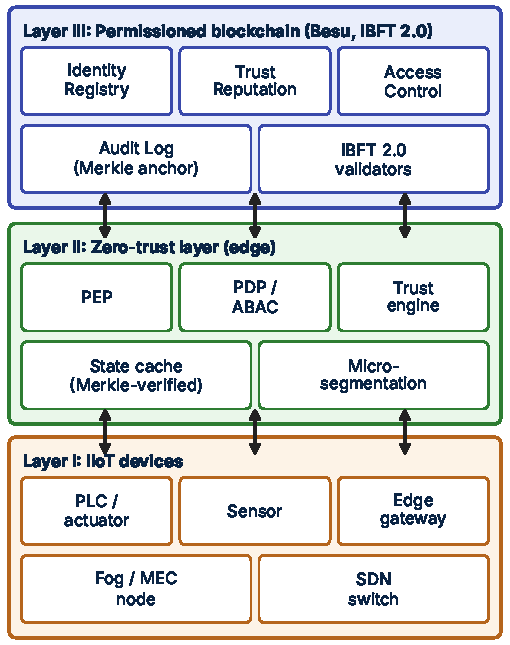
\includegraphics[width=1\columnwidth]{Figure_1}
\caption{Proposed BC-ZTA architecture: devices, edge/ZT layer, blockchain layer and contract services.}
\label{fig:1}
\end{figure}

\subsection{Edge and Zero-Trust Layers}

Sensors, actuators and PLCs hold an ECDSA key pair bound to a DID and sign every request with a timestamp and a nonce. Edge gateways terminate sessions, keep a local cache of identity, trust and policy state, and forward anomaly telemetry to the trust engine. On each gateway the PEP intercepts every request. The PDP verifies the signature, checks the DID against a cached, Merkle-verified registry entry, fetches the trust score and policy, and returns allow or deny. Micro-segmentation permits only flows that hold a valid, unexpired session~\cite{zanasi}, and the trust engine turns behavioural features (rate, protocol conformance, firmware attestation) into score proposals.

\subsection{Blockchain Layer}

A permissioned Hyperledger Besu network with IBFT 2.0 consensus is operated by plant, integrator and vendor validators; with \emph{n} validators it tolerates \emph{f} = $\lfloor$(\emph{n}$-$1)/3$\rfloor$ Byzantine nodes. Gateways are read-only clients that subscribe to events. Only authorised registrars, validators and the policy administrator send transactions.

\subsection{Identity, Trust and Access Control}

Each device is a DID with a public-key hash and a device class. A plant-authorised registrar submits registrations, which can be grouped into \emph{epochs}: the registrar commits the Merkle root of a batch, and a device later proves membership with a logarithmic-size path. Key rotation and revocation are single transactions that emit events. Trust scores lie in [0,100] and start at 70. A score changes only when a quorum of validators proposes the same value, updates are rate-limited, and an anomaly flag subtracts 20 points at once (floored at 0) until the device is re-evaluated. Policies are attribute-based: for each resource the administrator sets the allowed device-class range, a minimum trust score and a session TTL. A request is granted if the DID is active, the class is in range and the score meets the threshold, and the grant yields a session identifier that expires after the TTL or on explicit revocation.

\subsection{Smart Contracts}

\emph{IdentityRegistry} handles registration, key update, revocation, epoch commitment and membership checks. \emph{TrustReputation} handles quorum voting and the anomaly flag. \emph{AccessControl} holds policies, evaluates requests and grants or revokes sessions. \emph{AuditLog} stores per-event logs and Merkle batch anchors and verifies inclusion. Source code and tests are in the public repository.

\subsection{Continuous Verification}

Fig. 2 gives the workflow. Verification does not stop at login. Each request is checked again against the current cached trust, sessions are short, and the gateway refreshes cached entries every \emph{TTL} seconds, or at once when a \emph{DIDRevoked} or \emph{ScoreUpdated} event arrives. Audit records are hashed into a batch, and the Merkle root of that batch is anchored on-chain asynchronously (step 7), so logging never slows the response.

\begin{figure}[!tb]
\centering
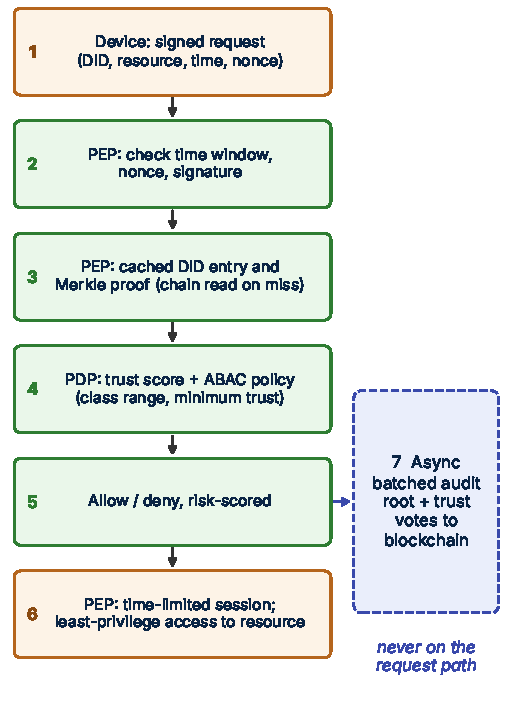
\includegraphics[width=1\columnwidth]{Figure_2}
\caption{Per-request verification workflow with cached state reads and asynchronous audit anchoring (step 7).}
\label{fig:2}
\end{figure}

A request is \emph{r} = (DID, resource, operation, \emph{t}, \emph{n}, $\sigma$): a timestamp, a nonce and the device's ECDSA signature over the other fields. The PEP accepts it only if (i) \textbar{}now $-$ \emph{t}\textbar{} $\leq$ $\Delta$ and \emph{n} is new within $\Delta$, which bounds replay; (ii) the DID is active in the cached registry, shown by a Merkle path against the latest committed epoch root or by a direct chain read on a miss; (iii) $\sigma$ verifies under the key whose hash is registered; and (iv) the PDP finds the trust score and policy satisfied. Otherwise the request is denied and an anomaly event is queued. The gateway also follows a fail-closed rule. If it cannot read the ledger, it keeps using a cached entry past its TTL for at most \emph{k}$\cdot$\emph{TTL} after the entry was last read (\emph{k} = 2 by default, parameter STALE\_FACTOR; we chose it so that one missed refresh does not lock a device out, while stale service stays below two cache lifetimes) and then denies with reason ``unavailable'' until the ledger is back; \emph{k} = 1 is the strict setting. A circuit breaker spares every request the read timeout while the source is down. The first cloud experiments (Sections 6.1--6.9) used an earlier prototype that denied as soon as a failed read followed TTL expiry (\emph{k} = 1), and the \emph{k} = 2 rule is evaluated in Section 6.10.

\subsection{Ledger Access, Revocation and Read Quorum}

A Merkle membership proof against an epoch root shows only that a DID was enrolled in that epoch. It stays valid after revocation, so it says nothing about freshness. Revocation is therefore enforced through the registry record (a revoked flag), which the gateway reads on a cache miss and which the \emph{DIDRevoked} event invalidates. A gateway also trusts the Besu node it reads from, and a compromised node could return stale or forged state. A gateway without a validator of its own can instead read from \emph{f} + 1 nodes pinned to the same block height and accept a state only if all answers agree: any \emph{f} + 1 matching answers include an honest node, and IBFT 2.0 has instant finality, so there are no forks to reconcile. The prototype implements this option (QUORUM = 2 for \emph{n} = 4); the default reads from one node, and the cost of the quorum is reported in Section 6.10.

\section{Use Case and Threat Model}

\subsection{Use Case}

Take a smart factory with several production cells. Each cell has PLCs and sensors behind one edge gateway. A remote vendor engineer needs time-limited maintenance access to one class of PLC, and a SCADA historian reads sensor data. The cells, the vendor and the integrator are separate administrative domains, and together they run the validators.

\subsection{Assets and Trust Assumptions}

The assets are device identities, policy and trust state, session tokens and audit records. We assume that most validators are honest (at most \emph{f} are Byzantine), that devices store their keys securely, and that gateways are trusted to enforce policy although any single one may be compromised.

\subsection{Adversary Model}

The adversary is a Dolev--Yao network attacker who can eavesdrop on, replay and inject messages. It may take over some devices (keys included) and one gateway. It may also include an insider with administrative credentials in one domain, though not enough to control a validator quorum.

\subsection{Threats and Countermeasures}

Table~\ref{tab:threat} maps threats to mechanisms. It shows what the design intends; entries marked in the table are not evaluated end to end, and Section 6.6 states what the cloud tests cover.

\begin{table}[!t]
\caption{Threats and countermeasures}
\label{tab:threat}
\footnotesize
\renewcommand{\arraystretch}{0.92}\setlength{\tabcolsep}{2pt}
\begin{tabular}{>{\raggedright\arraybackslash}p{0.224\linewidth}>{\raggedright\arraybackslash}p{0.292\linewidth}>{\raggedright\arraybackslash}p{0.431\linewidth}}
\toprule
\textbf{Threat} & \textbf{Attack} & \textbf{Countermeasure} \\
\midrule
Spoofing & Forged device identity & DID + ECDSA signature; Merkle-verified registry entry \\
Replay & Re-sent request & Timestamp + nonce window at PEP; session TTL \\
Lateral movement & Compromised device probes peers & Per-resource ABAC, short sessions (micro-segmentation: design only, not implemented) \\
Insider / tamper & Admin edits policy or logs & On-chain policy and Merkle-anchored audit; M-of-N admin possible (unit tests, Section 6.13) \\
Trust poisoning & False score votes & Quorum votes, rate limit; non-validators rejected (contract unit tests only) \\
Stale state & Use of revoked identity & Event-driven cache invalidation, bounded TTL \\
Ledger DoS & Flooding the chain & Off-path reads; batched writes; non-validators cannot write trust \\
\bottomrule
\end{tabular}
\end{table}

\subsection{Security Goals}

Authenticity of devices, least-privilege authorisation, revocation within a bounded delay, tamper-evident audit of anchored batches (attribution of a record to a signed request needs the v2 record format, which was tested locally only), and availability of access decisions during ledger congestion.

\subsection{Security Analysis}

We argue each goal under the assumptions of Sections 4.2--4.3 and four more: ECDSA over secp256k1 is unforgeable under chosen-message attack, Keccak-256 is collision- and second-preimage-resistant, gateway and device clocks differ by less than $\Delta$/2, and the enrolment authority registers only genuine devices. These are proof sketches, not machine-checked proofs; a ProVerif~\cite{blanchet} model of the request protocol remains future work.

\textbf{S1 Authenticity.} A request passes only if the signature recovers an address whose hash equals the key hash registered for the claimed DID. A forger without the device key must break signature unforgeability, and registering a new key needs the authority (\emph{updateKey}, \emph{registerDID}). \textbf{S2 Replay.} A replayed request fails if it is older than $\Delta$ or its nonce was already seen by \emph{the same gateway} within $\Delta$. The signed message carries no gateway identifier, so the same request can be replayed once at a different gateway within $\Delta$ unless nonce caches are shared or the gateway identity is added to the signed fields; we neither implemented nor tested this mitigation. \textbf{S3 Revocation.} Once the revocation transaction is final (IBFT 2.0 finality is instant), a gateway that sees the event stops accepting the device within the polling interval, and a gateway that misses it enforces the revocation when its cache entry expires, i.e. within \emph{TTL}. If consensus halts, the transaction cannot be finalised, so the bound runs from finalisation and not from submission (Section 6.10). \textbf{S4 Audit integrity.} Every batch root is anchored on-chain, so a stored record that is altered later no longer verifies, and changing an anchored root needs \emph{f} + 1 validators. Completeness is not guaranteed: a compromised gateway can drop records before they are anchored (and up to the 1 s anchoring interval is exposed on a crash), and the measured prototype's \emph{AuditLog} accepted anchors from any account (the released code restricts this to authorised gateways). \textbf{S5 Availability.} Decisions never wait for consensus and continue from cache for at most \emph{k}$\cdot$\emph{TTL} when the ledger is unreachable (Section 3.7). A gateway whose node is compromised can deny service or serve stale state unless the read quorum of Section 3.8 is used. \textbf{Gateway compromise.} A compromised gateway can approve any request and anchor batches that look valid: the ledger records what the gateway reports, not what happened, and the read quorum limits the state a gateway can be fed, not what it decides. A gateway that anchors two conflicting roots for the same batch leaves both on the ledger, so the conflict is visible (Section 6.13). \textbf{Staleness window.} If an attacker delays or blocks ledger events to a gateway, a revoked device keeps working until its cache entry expires, at most \emph{TTL}. If the attacker also controls the node the gateway reads from, that node can keep serving an old state with a proof that still verifies, and the bound no longer holds unless the \emph{f} + 1 read quorum is used; a stale answer then needs \emph{f} + 1 colluding nodes. Blocking the event feed leaves a gateway with TTL-only invalidation, which we did measure in E2: with a 10 s TTL a revocation took 6.6 s on average to take effect (Section 6.6). The bound for a compromised ledger node comes from argument only, and we did not run an eclipse or delay attack. \textbf{Administrator key.} In the measured prototype one policy-admin key could change policy and revoke sessions. The released code lets the admin role be handed to an M-of-N multisig contract (tested in unit tests, not measured), which removes the single key but raises the question of who the owners are. \textbf{Out of scope:} compromise of the enrolment authority, of \emph{f} + 1 validators or of a device key before revocation, and traffic analysis.

\section{Implementation and Experimental Methodology}

\subsection{Besu Blockchain Network}

We deployed a four-validator Hyperledger Besu v26.9.0 IBFT 2.0 network (\emph{f} = 1, block period 2 s, chain ID 2026, zero base fee, London EVM) in Docker on a GitHub-hosted 2-vCPU Linux runner for the contract-level micro-benchmark. All validators share that host, so network delay is negligible and CPU is contended. The end-to-end experiments ran separately on seven Google Cloud VMs (Section 5.6). A fresh network was started for each of 3 micro-benchmark repetitions, with contracts compiled by Solidity 0.8.20 (optimizer 200 runs, EVM ``london''). Five scenarios used pre-signed transactions from 8 worker wallets: S1 sequential write confirmation, S2 read latency (500 \emph{eth\_call} evaluations of \emph{AccessControl.evaluateRequest}), S3 per-event logging at 10--200 tx/s offered for 20 s, S4 batch anchoring at 1 tx/s, and S5 revocation visibility. Blocks were polled every 25 ms. Scripts, contracts and raw results are in the public repository listed under Data Availability.

\subsection{Smart Contracts}

The four core contracts total about 370 lines, and a fifth, optional contract lets a multisig take over the admin role. A Hardhat/Chai suite of 18 tests passes and covers registration, duplicate and unauthorised registration, revocation, key update, quorum scoring, score floor, rate limiting, non-validator rejection, access grant/deny, session expiry, epoch Merkle membership and audit batch inclusion proofs.

\subsection{End-to-End Prototype and Load Generator}

Besides the contract tests, we built the whole request path as running software (Node.js 20): a PEP/PDP service, a load generator and the baselines of Section 5.4. Every device owns a secp256k1 key and signs \emph{DID \textbar{} resource \textbar{} timestamp \textbar{} nonce}; its key hash and class are registered on-chain and its DID belongs to one Merkle epoch commitment. The PEP rejects timestamps older than 5 s and repeated nonces, recovers the signer, compares it with the registered key hash, checks the Merkle proof against the cached epoch root and evaluates the ABAC policy (device class 0--1, trust score $\geq$ 50). In BC-ZTA, identity, trust and policy state are read from Besu with \emph{eth\_call} on a cache miss and cached for 30 s. A block-polling subscription (20 ms) invalidates an entry when a \emph{DIDRevoked}, \emph{KeyUpdated} or \emph{ScoreUpdated} event is mined, every decision is hashed, and once per second the Merkle root of the pending batch is anchored with \emph{AuditLog.anchorBatch}. The load generator emulates N = 10, 25, 50, 100, 200 devices that send one request per second with staggered phases, after 5 s of warm-up and over a 20 s measurement window; requests are signed beforehand so the generator is not the bottleneck. Each request is sent at a fixed, pre-computed time whatever happened to earlier requests (open loop), so a slow decision does not delay later ones, and latency is measured from the moment of sending; scheduling lag of the generator was not recorded separately. PEP, directory server, load generator and the four validators run on separate machines (Section 5.6).

\subsection{Baselines}

(B1) \emph{Centralised PKI-IAM}: one lookup per request at a directory server on its own VM, whose responses are delayed by 40 ms with Linux \emph{tc netem} to model a remote central service (about 50 ms per lookup in total, Section 6.1). (B2) \emph{ABAC without blockchain}: a local attribute store at the PEP. (B3) \emph{Blockchain-only (sync)}: for every request the PEP reads state with \emph{eth\_call}, sends an \emph{AuditLog.logEvent} transaction (eight sender accounts) and replies only when the block containing it is observed. (B4) \emph{Keycloak}: a real Keycloak 26.4.0 issues each device an OpenID Connect access token whose claims carry its class, trust score and key hash, and the PEP calls the token-introspection endpoint~\cite{rfc7662} on every request; revocation disables the user. (B5) \emph{OpenLDAP}: a real slapd directory holding the same attributes, queried once per request~\cite{rfc4511}. B4 and B5 also run with a PEP-side decision cache (``cached'', TTL 10 s), which is the usual way to cut their latency. (P) \emph{BC-ZTA} as in Section 5.3. All systems use the same request format, signature check and policy, so differences come from where state is read and written.

\subsection{Performance Metrics}

(E1) End-to-end latency (mean, P95) from request send to decision, goodput (accepted requests per second), failures, and on-chain writes per second versus device count. (E2) Revocation enforcement delay: time from the revocation action until the PEP first denies the device. (E3) Security tests with 50 attempts each per run. (E4) Decision latency while the ledger is flooded with transactions. (E5) Decision latency, goodput and revocation enforcement while one of the four validators is stopped. Also gas per operation and, from the micro-benchmark, confirmation latency and ledger throughput.

\subsection{Distributed Deployment}

The end-to-end experiments E1--E5 ran on Google Cloud (us-central1-a) on seven VMs in one VPC without external addresses: four Besu validators (e2-medium, 2 vCPU, 4 GB, one validator each), a PEP/PDP host (e2-standard-2), the directory server for B1 (e2-small) and a controller (e2-standard-2) that runs the load generator and the experiment scripts and submits the on-chain transactions. Linux \emph{tc netem} delays all outgoing traffic of each validator VM by 5 ms, to stand for a plant-local validator network, and the responses of the directory server by 40 ms, to stand for a remote central service; all other delay is the real VM-to-VM delay. Each of the 5 repetitions started a freshly generated chain and restarted the PEP for every device count, and the repetitions ran one after another on the same VMs. The validator-failure test (E5) stops one validator container for 30 s while 50 devices are served. A single cloud zone is closer to independent hosts than a shared CI runner, but it is not an industrial network. Deployment scripts, configuration and raw results are in the public repository.

A second cloud run on the same VMs added Keycloak 26.4.0 (Docker, development mode, embedded H2 database) and OpenLDAP slapd (Debian 12 package) on the directory VM (B4, B5), their cached variants, a revocation test, a 25 s outage test, an open-loop PEP capacity test and the flood sweep of Section 6.9. Besu ran with a 2.5 GB heap for the flood sweep and all later runs; the first IAM repetition used the default 1 GB heap, which does not affect the PEP-side numbers.

All cloud runs used the first contract version, in which \emph{AuditLog} and \emph{grantSession} had no caller restriction (the hardening is described in Section 6.16), the unbound request signature and the per-event audit leaf; all used one resource with device-class and trust-score thresholds. Confidence intervals use the two-sided Student t value for n $-$ 1 degrees of freedom (4.30 for n = 3, 2.78 for n = 5) on the run means, which assumes roughly normal run-to-run variation and is wide for n = 3. The first cloud run (E1--E5) used e2-standard-2 PEP hosts and an unrecorded Besu heap. The IAM tests used 3 repetitions, the flood sweep 2, and the later runs of Sections 6.10--6.12 a 4-vCPU PEP host or no cloud VM at all; the run counts are given in each section.

\section{Results and Discussion}

\subsection{Authentication}

Table~\ref{tab:lat} and Fig. 3 show end-to-end latency (mean of 5 runs). At 50 devices BC-ZTA answers in 5.4 ms on average (P95 6.2 ms), versus 49.1 ms for the centralised PKI-IAM, 5.2 ms for the ledger-free ABAC store and 1382 ms for the synchronous blockchain. BC-ZTA is therefore 89\% faster than the centralised baseline. This gap is almost entirely the injected 40 ms delay, i.e. the one wide-area round trip that BC-ZTA removes from the request path; it would shrink or grow with that delay, which we did not sweep, so the percentage is not a general speed-up. BC-ZTA also costs about 0.2 ms more than a local store (Merkle verification, hashing and audit bookkeeping), and is about 255$\times$ faster than checking every request on-chain. Even at 10 devices, where the ledger is not saturated, the synchronous design needs 1172 ms because each request waits for a block.

\begin{table}[!t]
\caption{End-to-end latency (ms, mean $\pm$ 95\% CI of 5 runs; P95)}
\label{tab:lat}
\footnotesize
\renewcommand{\arraystretch}{0.92}\setlength{\tabcolsep}{2pt}
\begin{tabular}{>{\raggedright\arraybackslash}p{0.209\linewidth}>{\raggedright\arraybackslash}p{0.230\linewidth}>{\raggedright\arraybackslash}p{0.124\linewidth}>{\raggedright\arraybackslash}p{0.238\linewidth}>{\raggedright\arraybackslash}p{0.124\linewidth}}
\toprule
\textbf{System} & \textbf{Mean 50} & \textbf{P95 50} & \textbf{Mean 200} & \textbf{P95 200} \\
\midrule
PKI-IAM & 49.1 $\pm$ 0.2 & 50.0 & 49.0 $\pm$ 0.2 & 50.9 \\
ABAC & 5.2 $\pm$ 0.3 & 6.0 & 4.1 $\pm$ 0.2 & 5.1 \\
BC-only & 1382 $\pm$ 17 & 2272 & 12094 $\pm$ 6401 & 20757 \\
BC-ZTA & \textbf{5.4 $\pm$ 0.1} & \textbf{6.2} & \textbf{4.6 $\pm$ 0.2} & \textbf{5.8} \\
\bottomrule
\end{tabular}
\par\vspace{2pt}{\scriptsize Columns give the number of devices; PKI-IAM responses are delayed by 40 ms (netem). With 5 runs the differences discussed in the text exceed the confidence intervals by an order of magnitude; no hypothesis tests were run.}
\end{table}

\begin{figure}[!tb]
\centering
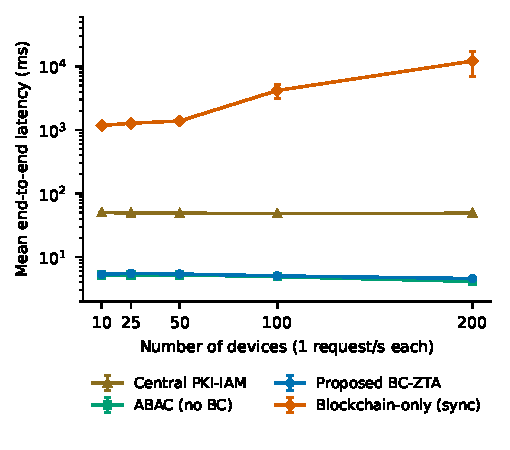
\includegraphics[width=1\columnwidth]{Figure_3}
\caption{Mean end-to-end latency versus number of devices (log scale; error bars: standard deviation of 5 runs; Table~\ref{tab:lat} gives 95\% confidence intervals).}
\label{fig:3}
\end{figure}

\subsection{Authorisation}

The proposed design makes policy decisions from the edge cache. The measured cache-hit ratio was 96\% (one miss per device per 30 s TTL), so 50 devices caused only 50 chain reads for about 1,250 requests; each miss costs one batched \emph{eth\_call} of 5.4 ms in the micro-benchmark. The PEP used 0.29 CPU cores at 50 devices and 0.65 at 200, against 0.53 for the local store. Every decision is covered by the audit batch: in the 200-device runs about 5,000 decisions per run were anchored in roughly 25 transactions. On-chain evaluation costs 44,685 gas as an estimate, but because it is a read, no fee or block wait is incurred.

\subsection{Blockchain Throughput}

The Besu micro-benchmark gave the following. Write confirmation takes 1522 ms on average at 10 tx/s (P95 2439 ms), close to the 2 s block period; a transaction submitted just after a block, as in the phase-locked sequential tests S1/S5, waits about 1980 ms. Reads cost 5.4 ms (P95 10.9 ms). Committed throughput tracks the offered load up to 50 tx/s (46.5 tx/s) but saturates near 60 tx/s on this host: at 100 and 200 tx/s offered only 62.7 and 59.1 tx/s commit and 43\% of transactions at 200 tx/s were not confirmed within 60 s. Batch anchoring at 1 tx/s confirmed all 60 anchors in 941 ms on average. Because all validators share one 2-vCPU host, 60 tx/s is a lower bound: on the seven-VM deployment the synchronous baseline committed up to 112 tx/s (Section 6.5), almost twice as much.

\subsection{Resource Utilisation}

Measured gas per operation is listed in Table~\ref{tab:gas}. Registering a device costs 55,682 gas, whereas committing an epoch root costs 75,469 gas independent of batch size. Logging one event on-chain costs 182,008 gas, while anchoring a batch costs 134,747 gas, i.e. about 135 gas per record for a 1,000-record batch ($\approx$1351$\times$ cheaper); the saving is proportional to the batch size and is $\approx$68$\times$ for the 50 records per batch of the 50-device experiments and $\approx$270$\times$ for 200 devices. At 400 devices and 1 event/s the calculation gives 34.6 M events/day: 6636 MB/day of ledger growth with per-event logging (192 B/entry) versus 13.8 MB/day with batch anchoring. Device-side CPU and memory were not measured. An IOTA-based DID study reports about 175\% CPU on a Raspberry Pi against about 22\% on a conventional computer while generating a DID~\cite{ramirez}, which is why we limit devices to one signature and a hash proof.

\begin{table}[!t]
\caption{Measured gas per contract operation}
\label{tab:gas}
\footnotesize
\renewcommand{\arraystretch}{0.92}\setlength{\tabcolsep}{2pt}
\begin{tabular}{>{\raggedright\arraybackslash}p{0.623\linewidth}>{\raggedright\arraybackslash}p{0.335\linewidth}}
\toprule
\textbf{Operation} & \textbf{Gas} \\
\midrule
IdentityRegistry.registerDID & 55,682 \\
IdentityRegistry.commitEpoch & 75,469 \\
IdentityRegistry.revokeDID & 49,550 \\
AccessControl.setPolicy & 49,731 \\
AccessControl.grantSession & 71,689 \\
TrustReputation.updateScore (quorum) & 124,772 \\
TrustReputation.flagAnomaly & 95,868 \\
AuditLog.logEvent (per event) & 182,008 \\
AuditLog.anchorBatch (per batch) & 134,747 \\
\bottomrule
\end{tabular}
\par\vspace{2pt}{\scriptsize Hardhat EVM (london), optimizer 200 runs; first-use storage costs included.}
\end{table}

\subsection{Scalability}

Fig. 4 shows goodput and on-chain write load against device count. Central PKI-IAM, ABAC and BC-ZTA served every request up to 200 devices with no failures. The synchronous blockchain kept up to 50 devices (goodput 50 req/s, 1.4 s mean latency) and at 100 devices (100 req/s, 4.2 s), but at 200 devices only 40\% of the requests were answered in time, goodput fell to 81 req/s and 4331 requests (summed over 5 runs) failed or timed out. Its on-chain write rate (100 tx/s at 100 and 112 tx/s at 200 devices) is the measured ledger ceiling of this deployment, whereas BC-ZTA writes about 1.0 tx/s regardless of the number of devices. The latency of BC-ZTA stays flat from 10 to 200 devices (5.4 to 4.6 ms mean, P95 at most 6.4 ms), and the PEP used 0.65 of its two vCPUs at 200 devices, so neither the ledger nor the PEP was the limit at this load; larger populations were not tested. For comparison, a sharded design reaches 2,500 TPS at 700 nodes~\cite{salim}; our approach instead lowers the required write rate.

\begin{figure}[!tb]
\centering
\begin{subfigure}{\columnwidth}\centering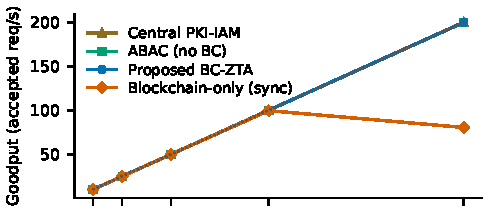
\includegraphics[width=0.95\linewidth]{Figure_4a}\caption{}\end{subfigure}
\begin{subfigure}{\columnwidth}\centering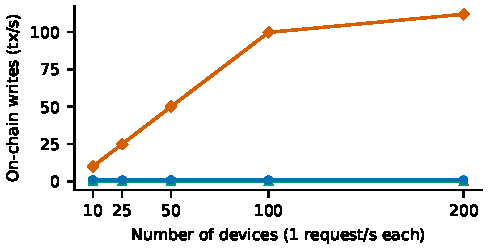
\includegraphics[width=0.95\linewidth]{Figure_4b}\caption{}\end{subfigure}
\caption{(a) Goodput and (b) on-chain writes per second versus number of devices. The dotted line is the offered load and lies under the BC-ZTA line. The legend in (a) applies to (b).}
\label{fig:4}
\end{figure}

\subsection{Negative Security Tests}

Table~\ref{tab:sec} lists the security tests run against the BC-ZTA prototype (5 runs, 50 attempts per test and run). All legitimate requests were accepted (no false rejects), and none of the forged, replayed, stale, unregistered, tampered, class-violating or low-trust requests was accepted. These are negative tests: each checks that one malformed request is refused by one mechanism. They do not model an adversary who compromises a gateway, holds the admin key, eclipses a node, controls several score voters or runs many fake devices. Those cases are covered by the argument in Section 4.6 and, for operator tampering with the audit trail, by the local experiment of Section 6.13; they were not tested on the cloud deployment. For a revoked device, 0 requests were accepted after the revocation transaction was confirmed, and the first denial came 15 ms after confirmation or sooner. Fig. 5 shows the revocation enforcement delay of each system: with event-driven invalidation BC-ZTA enforces a revocation after 1.25 s on average (worst case 2.23 s), about one block period and independent of the TTL, whereas TTL-only refresh with a 10 s TTL needs 6.6 s on average (worst case 11.5 s). The centralised and local baselines revoke in 57 ms and 22 ms because they hold the state in one place (the ABAC samples are bimodal, about 7 or 57 ms, which we did not trace); the blockchain-only value (1.35 s) includes the request that was in flight when the revocation was issued.

\begin{table}[!t]
\caption{Negative security tests on the BC-ZTA prototype (5 runs)}
\label{tab:sec}
\footnotesize
\renewcommand{\arraystretch}{0.92}\setlength{\tabcolsep}{2pt}
\begin{tabular}{>{\raggedright\arraybackslash}p{0.565\linewidth}>{\raggedright\arraybackslash}p{0.191\linewidth}>{\raggedright\arraybackslash}p{0.191\linewidth}}
\toprule
\textbf{Test} & \textbf{Attempts} & \textbf{Accepted} \\
\midrule
Legitimate requests (control) & 250 & 250 \\
Forged signature & 250 & 0 \\
Replayed request & 250 & 0 \\
Stale timestamp & 250 & 0 \\
Unregistered DID & 250 & 0 \\
Tampered Merkle proof & 250 & 0 \\
Class outside policy & 250 & 0 \\
Trust score below threshold & 250 & 0 \\
\bottomrule
\end{tabular}
\par\vspace{2pt}{\scriptsize For the control row, Accepted is the desired outcome; for all other rows it must be 0.}
\end{table}

\begin{figure}[!tb]
\centering
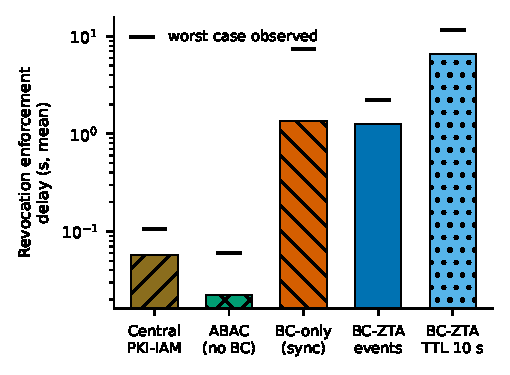
\includegraphics[width=1\columnwidth]{Figure_5}
\caption{Revocation enforcement delay (mean, log scale; marks: worst case observed).}
\label{fig:5}
\end{figure}

\subsection{Availability under Validator Failure}

E5 stops one of the four validators for 30 s while 50 devices are served and one device is revoked during the outage. IBFT 2.0 with four validators tolerates \emph{f} = 1 faulty validator and the PEP decides from its cache, so decisions should be unaffected. The test confirms this: all 3500 requests were answered and accepted (mean 5.4 ms, P95 6.8 ms, none late or failed), the revoked device was denied 1.76 s after the revocation was submitted, and the PEP kept anchoring audit batches (73 of 75 anchor transactions were confirmed when the statistics were read). Only one failure of one validator for 30 s was tested; network partitions, Byzantine validators and the loss of two validators were not.

\subsection{Comparison with Production IAM Services}

To replace the simple directory of B1 with real products, we added Keycloak 26.4 as an OpenID Connect token-introspection service~\cite{rfc7662} (B4) and OpenLDAP slapd as a directory queried once per request~\cite{rfc4511} (B5), each on the directory VM behind the same 40 ms netem delay, plus a variant of each with a 10 s decision cache at the PEP (``cached''). All five systems share the PEP, signatures and policy. Table~\ref{tab:iam} gives the results (3 repetitions). At 25 and 100 devices the uncached products need 48.3 ms (Keycloak) and 46.8 ms (OpenLDAP) per decision because every request crosses the emulated WAN, against 6.3 ms for BC-ZTA, which is 8$\times$ and 7$\times$ faster. Most of that gap is the removed WAN round trip: with a PEP-side cache the products reach 9.8--9.5 ms mean latency, and only their P95 (48 ms, one miss per device per TTL) stays WAN-bound. The cached products enforce a revocation only once the cache expires (mean 5.5 s, worst case 9.5 s for the 10 s TTL), whereas BC-ZTA's event-driven invalidation did so in 1.2 s in this run and 1.3 s in the five-run test of Section 6.6 (worst case 2.2 s), at the same low latency. The uncached products revoke faster, in 84 ms (Keycloak) and 72 ms (OpenLDAP), because the central service is consulted on every request. A plant that needs sub-second revocation must use the uncached products or a shorter block period.

\begin{table}[!t]
\caption{Production IAM baselines: latency (mean / P95, ms) and revocation delay}
\label{tab:iam}
\footnotesize
\renewcommand{\arraystretch}{0.92}\setlength{\tabcolsep}{2pt}
\begin{tabular}{>{\raggedright\arraybackslash}p{0.324\linewidth}>{\raggedright\arraybackslash}p{0.152\linewidth}>{\raggedright\arraybackslash}p{0.152\linewidth}>{\raggedright\arraybackslash}p{0.152\linewidth}>{\raggedright\arraybackslash}p{0.145\linewidth}}
\toprule
\textbf{System} & \textbf{25 dev.} & \textbf{100 dev.} & \textbf{200 dev.} & \textbf{Revoc. (s)} \\
\midrule
Keycloak & 49.7 / 52 & 48.3 / 50 & 123.4 / 304 & 0.08 \\
Keycloak, cached & 10.2 / 49 & 9.8 / 48 & 12.4 / 56 & 5.55 \\
OpenLDAP & 47.3 / 49 & 46.8 / 49 & 77.2 / 243 & 0.07 \\
OpenLDAP, cached & 10.1 / 47 & 9.5 / 47 & 10.6 / 50 & 5.20 \\
BC-ZTA & \textbf{6.4 / 7} & \textbf{6.3 / 8} & 117.2 / 255 & \textbf{1.18} \\
\bottomrule
\end{tabular}
\par\vspace{2pt}{\scriptsize Mean of 3 repetitions; 40 ms netem delay on the IAM services; revocation: 8 devices per run, mean of 24; cache TTL 10 s.}
\end{table}

\begin{figure*}[!t]
\centering
\begin{subfigure}{0.49\textwidth}\centering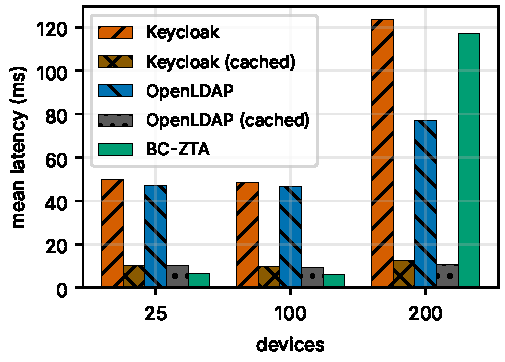
\includegraphics[width=\linewidth]{Figure_6a}\caption{}\end{subfigure}\hfill
\begin{subfigure}{0.49\textwidth}\centering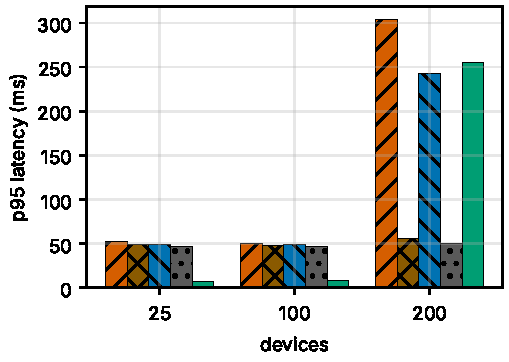
\includegraphics[width=\linewidth]{Figure_6b}\caption{}\end{subfigure}
\caption{(a) Mean and (b) P95 latency of Keycloak, OpenLDAP, their cached variants and BC-ZTA. The legend in (a) applies to (b).}
\label{fig:6}
\end{figure*}

At 200 devices (one request per second each) the PEP, a single Node.js process on a 2-vCPU VM, nears its own capacity: BC-ZTA (117 ms mean, 255 ms P95) and uncached Keycloak (123 ms) degrade alike, while the cached products do not. In the Section 6.1 run the same configuration decided in 4.6 ms, so this point sits at the saturation edge and varies between runs. It is a limit of our single-process PEP, not of the architecture, since PEPs are stateless and can be replicated. An open-loop capacity test (200--1,600 req/s, 3 repetitions) shows goodput saturating at about 246--291 req/s for all three systems, with P95 latency of several seconds beyond it, so per-PEP capacity is set by signature verification and not by the IAM backend.

Table~\ref{tab:outage} reports the outage test: the central service is stopped 20 s into a 100 s run with 100 devices and restarted at 45 s. Without Keycloak or OpenLDAP no new decisions are possible: 0\% of requests were granted during the outage with both uncached products and 4\% with the cached variants, whose entries expired within 2 s of the stop (most entries had already expired). Service resumed 1 s after restarting OpenLDAP and 14 s after restarting Keycloak (JVM start-up). The PEP of BC-ZTA contacts no central service and granted 100\% throughout (Fig. 7). This test removes a service that BC-ZTA does not use, and a design that caches decisions and receives pushed revocations from the same directory would also survive a short outage, so the fairer comparison is the loss of each design's own state source (Section 6.10). We did not test clustered Keycloak or OpenLDAP. The test shows the single point of failure that BC-ZTA removes, not that central IAM cannot be made highly available.

\begin{table}[!t]
\caption{Central-service outage (25 s, 100 devices, 3 runs)}
\label{tab:outage}
\footnotesize
\renewcommand{\arraystretch}{0.92}\setlength{\tabcolsep}{2pt}
\begin{tabular}{>{\raggedright\arraybackslash}p{0.401\linewidth}>{\raggedright\arraybackslash}p{0.273\linewidth}>{\raggedright\arraybackslash}p{0.273\linewidth}}
\toprule
\textbf{System} & \textbf{Granted during outage (\%)} & \textbf{Recovery after restart (s)} \\
\midrule
Keycloak & 0 & 14 \\
Keycloak, cached & 4 & 14 \\
OpenLDAP & 0 & 1 \\
OpenLDAP, cached & 4 & 1 \\
BC-ZTA & \textbf{100} & \textbf{0} \\
\bottomrule
\end{tabular}
\par\vspace{2pt}{\scriptsize Service stopped at 20 s and restarted at 45 s of a 100 s run; BC-ZTA has no central service (Keycloak was stopped on the directory VM, but BC-ZTA does not use it).}
\end{table}

\begin{figure}[!tb]
\centering
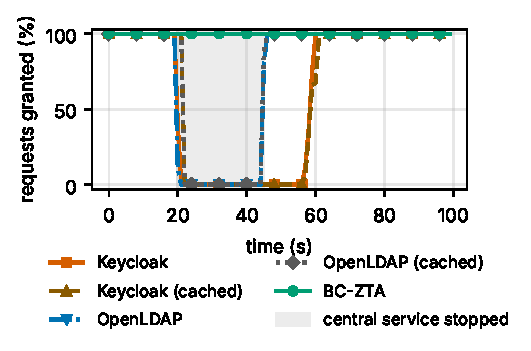
\includegraphics[width=1\columnwidth]{Figure_7}
\caption{Fraction of requests granted over time while the central IAM service is stopped (shaded) and restarted.}
\label{fig:7}
\end{figure}

\subsection{Ledger Flood Sweep}

To test ledger flooding we swept the offered rate of audit-log transactions from 0 to 1,200 tx/s (16 spam wallets, pre-signed transactions sent in nonce order, 20 s per rate after a 5 s warm-up, 50 devices at 1 request/s, 2 repetitions), once with BC-ZTA and once with the synchronous design, which writes every decision as a transaction on the same ledger (Fig. 8). The committed rate saturates at about 193 tx/s for BC-ZTA and 215 tx/s for the synchronous design (peak at 200--400 tx/s offered) and then declines, to 106 and 152 tx/s at 1,200 offered, because Besu rejects most of the excess (``nonce too distant'' and, at the highest rate, ``transaction pool not enabled''; 50266 of 64802 submissions in the BC-ZTA run). The access latency of BC-ZTA does not follow: its mean stays at 5.8--6.3 ms and its P95 at no more than 7.9 ms with every request answered, since decisions never wait for the ledger. The mean latency of the synchronous design climbs from 1.6 s with an idle ledger to 24 s at 1,200 tx/s (P95 30 s), and 7\% of its requests fail at the highest rate. A flood thus denies service to ledger-bound designs but only delays BC-ZTA's audit anchoring and revocation visibility, which we did not measure under flood.

\begin{figure*}[!t]
\centering
\begin{subfigure}{0.49\textwidth}\centering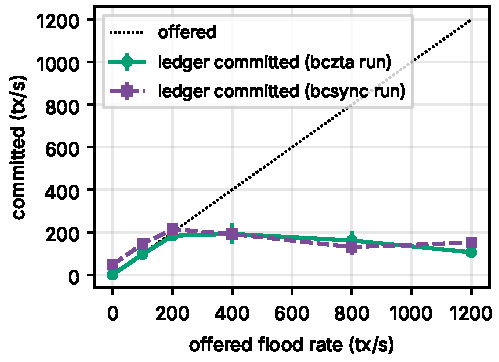
\includegraphics[width=\linewidth]{Figure_8a}\caption{}\end{subfigure}\hfill
\begin{subfigure}{0.49\textwidth}\centering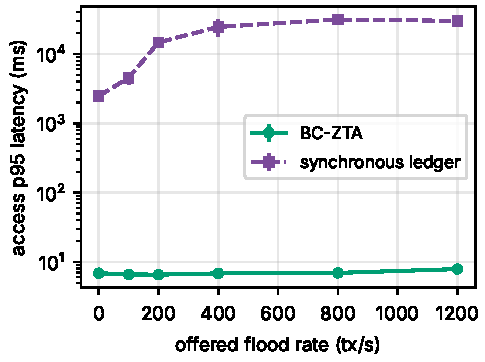
\includegraphics[width=\linewidth]{Figure_8b}\caption{}\end{subfigure}
\caption{(a) Committed ledger rate and (b) access P95 latency versus offered flood rate.}
\label{fig:8}
\end{figure*}

The flood generator targets the validator that the PEP also reads from. We raised the Besu heap to 2.5 GB after the default 1 GB ran out of memory in the synchronous run at 400 tx/s. We did not test a flood against all validators, an attacker with more accounts, or a longer flood. The committed rate of 100--215 tx/s is specific to our four validators, 2 s block period and two vCPUs per validator.

\subsection{Robustness: Push Revocation, Read Quorum, Fail-Closed Bound, Consensus Halt and Scaling}

The comparison with Keycloak and OpenLDAP leaves open whether the ledger is needed for what BC-ZTA does well. We therefore added baseline B6, a central directory (40 ms WAN delay) whose answers the PEP caches for 30 s and which pushes each revocation to the PEP over a server-sent-event stream, i.e. event-driven invalidation without a blockchain, and BC-ZTA with a read quorum of \emph{f} + 1 = 2 validators (Section 3.8). The experiments ran 3 times, each on a fresh network, with the PEP host enlarged to e2-standard-4 (4 vCPU); Table~\ref{tab:push} gives the results. B6 decides in 3.9 $\pm$ 0.4 ms at 100 devices against 4.2 $\pm$ 0.4 ms for BC-ZTA, so the two are close for access latency: the difference (BC-ZTA minus B6) is 0.2 ms (95\% CI $-$0.1 to 0.6 ms) at 100 devices and 0.4 ms (95\% CI 0.1 to 0.6 ms) at 200 devices, where BC-ZTA is measurably, though slightly, slower; the upper bound of the interval is 0.7 ms or less at 25, 100 and 200 devices (Student \emph{t}, 3 runs each). We set no equivalence margin beforehand, so this is an interval estimate, not an equivalence test. B6 enforces a revocation after 109 ms on average (worst case 154 ms), which is 11$\times$ faster than BC-ZTA with quorum (1.2 s, worst case 2.1 s), because BC-ZTA must wait for a block. The read quorum changes the mean latency at 100 devices from 4.2 $\pm$ 0.4 to 4.6 $\pm$ 1.1 ms, since only cache misses read from two nodes, and no quorum mismatch occurred in the runs. A trusted central operator who pushes revocations thus matches BC-ZTA's latency and revokes faster. What the ledger adds is that no single operator holds identity, policy and audit records, and that the other consortium members can verify anchored audit. Where one operator is acceptable, B6 is the simpler design.

\begin{table}[!t]
\caption{Central directory with push revocation (B6) and read quorum (3 runs)}
\label{tab:push}
\footnotesize
\renewcommand{\arraystretch}{0.92}\setlength{\tabcolsep}{2pt}
\begin{tabular}{>{\raggedright\arraybackslash}p{0.285\linewidth}>{\raggedright\arraybackslash}p{0.152\linewidth}>{\raggedright\arraybackslash}p{0.152\linewidth}>{\raggedright\arraybackslash}p{0.152\linewidth}>{\raggedright\arraybackslash}p{0.183\linewidth}}
\toprule
\textbf{System} & \textbf{25 dev.} & \textbf{100 dev.} & \textbf{200 dev.} & \textbf{Revoc. (ms)} \\
\midrule
B6 push & 4.7 $\pm$ 0.3 & 3.9 $\pm$ 0.4 & 3.6 $\pm$ 0.3 & 109 \\
BC-ZTA & 4.5 $\pm$ 0.5 & 4.2 $\pm$ 0.4 & 4.0 $\pm$ 0.3 & 1252 \\
BC-ZTA, quorum 2 & 4.6 $\pm$ 0.2 & 4.6 $\pm$ 1.1 & 4.0 $\pm$ 0.5 & 1162 \\
\bottomrule
\end{tabular}
\par\vspace{2pt}{\scriptsize Mean latency (ms) $\pm$ 95\% CI of 3 runs; revocation: mean of 24 (B6) and 24 (quorum) samples; the BC-ZTA value is from the five-run test of Section 6.6. TTL 30 s (latency), 10 s (revocation).}
\end{table}

Section 6.8 stopped Keycloak or OpenLDAP, which BC-ZTA does not use. The fair test is the loss of each design's own state source under the same cache policy (TTL 10 s, serve-stale bound 2$\cdot$TTL = 20 s, 50 devices): the PEP of BC-ZTA is cut off from its ledger node with a firewall rule (\emph{iptables} DROP) for 50 s, and the directory of B6 is stopped for the same time (Table~\ref{tab:cut}, Fig. 9, 3 runs). The two behave alike. Requests are granted from cache and then from stale state (89\% and 100\% granted in the first 10 s after the loss), the granted fraction falls to 0\% and 0\% once the last read is older than 20 s, and service resumes 1 s and 1 s after the source returns. The first denials come 9 s (BC-ZTA) and 12 s (B6) after the loss, not after 20 s, because the bound of each entry runs from its own last successful read, up to one TTL before the loss. The first reads that hit the unreachable ledger also wait for the 2.5 s read timeout, so BC-ZTA grants slightly less than B6 in the first window. The ledger therefore gives no extra availability in this test, since any cache with a stale bound behaves the same way in a short outage. BC-ZTA state sits on four validators, so the PEP could read from another node (we did not implement failover); the B6 directory is a single service unless replicated.

\begin{table}[!t]
\caption{Loss of the state source (TTL 10 s, stale bound 20 s, 3 runs)}
\label{tab:cut}
\footnotesize
\renewcommand{\arraystretch}{0.92}\setlength{\tabcolsep}{2pt}
\begin{tabular}{>{\raggedright\arraybackslash}p{0.332\linewidth}>{\raggedright\arraybackslash}p{0.103\linewidth}>{\raggedright\arraybackslash}p{0.103\linewidth}>{\raggedright\arraybackslash}p{0.122\linewidth}>{\raggedright\arraybackslash}p{0.111\linewidth}>{\raggedright\arraybackslash}p{0.144\linewidth}}
\toprule
\textbf{System (source lost)} & \textbf{Before} & \textbf{$\leq$ TTL} & \textbf{TTL--2TTL} & \textbf{\textgreater{} 2TTL} & \textbf{Restored} \\
\midrule
BC-ZTA (ledger node) & 100 & 89 & 15 & 0 & 100 \\
B6 (directory) & 100 & 100 & 20 & 0 & 100 \\
\bottomrule
\end{tabular}
\par\vspace{2pt}{\scriptsize Requests granted (\%) in the windows after the loss of the state source; windows are relative to the time of the loss.}
\end{table}

\begin{figure}[!tb]
\centering
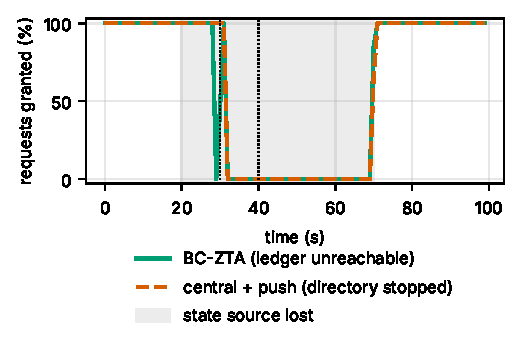
\includegraphics[width=1\columnwidth]{Figure_9}
\caption{Requests granted while the state source is lost (shaded); dotted lines: TTL and 2$\cdot$TTL after the loss.}
\label{fig:9}
\end{figure}

To test the consensus assumption we stopped two of the four validators for 40 s (IBFT 2.0 needs three, so block production halts) while 50 devices were served, and revoked a device 5 s after the stop. The PEP kept answering: 100\% of requests were granted during the halt, because the cache and the reachable node serve the last committed state. The revoked device, however, stayed accepted until consensus resumed and the transaction was mined. Enforcement came 73.4 s after the validators were restarted and 108.4 s after submission (3 runs). The staleness bound of BC-ZTA therefore runs from finalisation of the revocation and not from its submission, so a consensus halt is a window in which revocations cannot take effect; a central directory is not affected by this particular failure. The delay is far longer than the halt itself (40 s): block production stayed frozen for 73 s after the restart. We did not test the cause. It fits the IBFT 2.0 rule that the timeout of a round doubles after each failed round (base 4 s here), so the validators needed one long round to agree again. Shorter base timeouts or supervised restarts would cut the delay, and an operator who needs bounded revocation during a halt must also keep a short-lived local deny list at the PEP.

Finally, per-PEP capacity is not a limit of the architecture if gateways are replicated. We ran k = 1, 2, 4 PEP processes on one 4-vCPU VM, with devices sharded across them, and raised the offered rate (Fig. 10, Table~\ref{tab:scale}). The highest offered rate served without any failed request and with a P95 below 50 ms was 200 req/s for k = 1, 400 req/s for k = 2, 400 req/s for k = 4. At 800 req/s offered, k = 1 is overloaded (goodput 457 req/s, P95 8.5 s) and k = 2 is overloaded (goodput 706 req/s, P95 7.2 s), whereas k = 4 delivers 770 req/s (96\% of the offered rate) at a P95 of 436 ms while using 2.4 cores of the 4-vCPU VM. Beyond that, goodput falls as the offered rate rises (overload collapse: requests queue behind signature verification and time out), so each gateway must stay below its knee, which an admission limit or load balancer would enforce. Scale-out was measured on one host; across hosts the shared state is the ledger, which is read once per device per TTL.

\begin{table*}[!t]
\caption{PEP scale-out (BC-ZTA, 3 runs)}
\label{tab:scale}
\footnotesize
\renewcommand{\arraystretch}{0.92}\setlength{\tabcolsep}{2pt}
\begin{tabular}{>{\raggedright\arraybackslash}p{0.140\linewidth}>{\raggedright\arraybackslash}p{0.192\linewidth}>{\raggedright\arraybackslash}p{0.227\linewidth}>{\raggedright\arraybackslash}p{0.175\linewidth}>{\raggedright\arraybackslash}p{0.192\linewidth}}
\toprule
\textbf{PEPs} & \textbf{Clean rate (req/s)} & \textbf{Goodput at 800 (req/s)} & \textbf{P95 at 800 (ms)} & \textbf{CPU cores at 800} \\
\midrule
1 & 200 & 457 & 8464 & 0.7 \\
2 & 400 & 706 & 7172 & 1.2 \\
4 & 400 & 770 & 436 & 2.4 \\
\bottomrule
\end{tabular}
\par\vspace{2pt}{\scriptsize Clean rate = highest offered rate with no failed request and P95 \textless{} 50 ms; one VM; load generator on a separate VM; mean of the runs.}
\end{table*}

\begin{figure*}[!t]
\centering
\begin{subfigure}{0.49\textwidth}\centering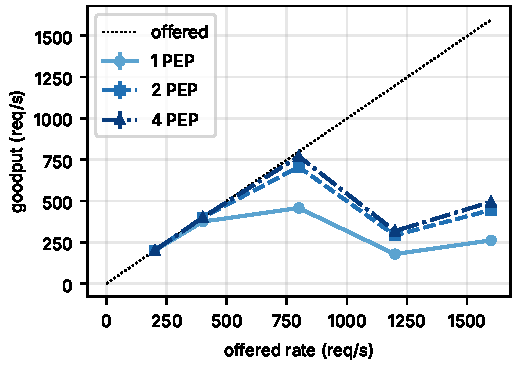
\includegraphics[width=\linewidth]{Figure_10a}\caption{}\end{subfigure}\hfill
\begin{subfigure}{0.49\textwidth}\centering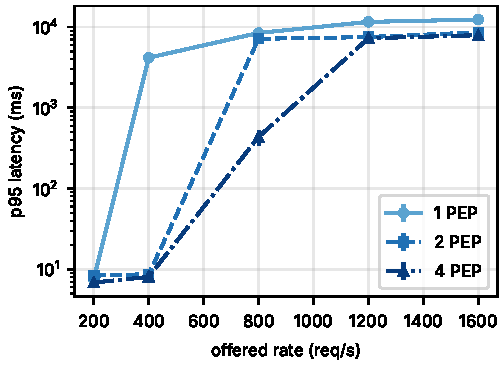
\includegraphics[width=\linewidth]{Figure_10b}\caption{}\end{subfigure}
\caption{(a) Goodput and (b) P95 latency versus offered request rate for 1, 2 and 4 PEP processes.}
\label{fig:10}
\end{figure*}

\subsection{Independent Verification of the Audit Trail}

A ledger-anchored audit log is only useful if someone outside the operator can check it. We tested this locally, without the cloud, with the same sorted-pair Merkle construction and keccak hashing as \emph{AuditLog.anchorBatch}. For batches of 50 to 5,000 synthetic audit records, we computed the root and treated it as the value anchored on the ledger. An adversary who controls the stored log then changed one record, deleted one, inserted one, or swapped two adjacent ones (100 trials per case and size). The verifier recomputes the root from the log it is given and compares it with the anchored root. Table~\ref{tab:audit} shows that modification, deletion and insertion were caught in every trial at every batch size. Recomputing the whole batch took 1.4 ms for 50 records and 155 ms for 5,000 on one core, and a verifier interested in one record needs a proof of 192--416 bytes and 0.11--0.25 ms. A forged record presented with an honest proof was never accepted (0 of 100).

Two limits matter. First, swapping two adjacent records was caught in only 42--61\% of the trials. Sorted-pair hashing makes the root of two sibling leaves independent of their order, so the root commits to the set of records and not to their order. Order can be checked only if every record carries a sequence number that the verifier inspects; the measured prototype's records carry a timestamp and a nonce, not a counter (the v2 format below adds one). Second, the anchor covers a record only from the moment its batch is closed and anchored. A record falsified before that, a batch whose root was never anchored, and a log the operator refuses to hand over are outside what the ledger proves: it shows that a root existed at a given block, not that the log is complete. A central database log without an external commitment gives a third party nothing to compare against, so a rewritten row is undetectable by construction (we did not measure this case). This test shows that the tamper-evidence claim holds for the mechanism; it does not compare BC-ZTA with a transparency log or with an operator-published Merkle log of the kind in~\cite{yagiz26}, which offer similar evidence without consensus. What the ledger adds over these is a publication medium that no single party controls.

We then tested the remedy for the ordering gap. In record format v2 (\emph{AUDIT\_V2}, default off in the PEP) each record also carries a gateway identifier, a per-gateway sequence number, the decision and a hash of the device signature, and the verifier additionally requires the sequence numbers of a presented batch to run 0 to n $-$ 1 in order. In the same local setting (100 trials per case and size, batches of 50 to 5000), modification, deletion, insertion, adjacent swaps and swaps followed by renumbering were detected in 2500 of 2500 trials, with no false alarm on the untouched batch. The hash of the device signature makes a record attributable to a signed request, so a gateway cannot later claim it never saw one; it does not prove that the gateway recorded every request it received, and a gateway authorised to anchor can still omit records. These formats were tested locally and were not part of the cloud runs.

\begin{table}[!t]
\caption{Detection of tampering with anchored audit batches (100 trials per cell)}
\label{tab:audit}
\footnotesize
\renewcommand{\arraystretch}{0.92}\setlength{\tabcolsep}{2pt}
\begin{tabular}{>{\raggedright\arraybackslash}p{0.102\linewidth}>{\raggedright\arraybackslash}p{0.112\linewidth}>{\raggedright\arraybackslash}p{0.112\linewidth}>{\raggedright\arraybackslash}p{0.112\linewidth}>{\raggedright\arraybackslash}p{0.112\linewidth}>{\raggedright\arraybackslash}p{0.130\linewidth}>{\raggedright\arraybackslash}p{0.102\linewidth}>{\raggedright\arraybackslash}p{0.112\linewidth}}
\toprule
\textbf{Batch} & \textbf{Modify} & \textbf{Delete} & \textbf{Insert} & \textbf{Swap} & \textbf{Full (ms)} & \textbf{Proof (B)} & \textbf{Proof (ms)} \\
\midrule
50 & 100/100 & 100/100 & 100/100 & 50/100 & 1.4 & 192 & 0.11 \\
100 & 100/100 & 100/100 & 100/100 & 61/100 & 2.6 & 224 & 0.13 \\
500 & 100/100 & 100/100 & 100/100 & 48/100 & 14.1 & 288 & 0.17 \\
1000 & 100/100 & 100/100 & 100/100 & 52/100 & 29.3 & 320 & 0.19 \\
5000 & 100/100 & 100/100 & 100/100 & 42/100 & 155.1 & 416 & 0.25 \\
\bottomrule
\end{tabular}
\par\vspace{2pt}{\scriptsize Detected/trials. Run on a 2-vCPU container with Node v22.23.4, not on the cloud VMs; the log and its proofs are held by the adversary, the root by the ledger.}
\end{table}

\subsection{Registry Size}

The end-to-end runs used up to 200 devices. To see whether proof handling would limit larger sites, we measured the Merkle epoch tree of the device registry from 1,000 to 1,000,000 entries in the same local test. The proof grows from 320 to 640 bytes (depth 10 to 20) and one proof takes 0.18 to 0.43 ms to verify on one core, which is 2,307--5,474 verifications per second per core with a JavaScript hash. A PEP that verifies a proof on every cache miss therefore pays well under a millisecond even at one million devices, and the cost grows with the logarithm of the registry. The costs that grow faster are building the tree, which the registrar does once per epoch off the request path (27 s for 1,000,000 entries on one core), and the cache itself. These numbers cover proof handling only. They contain no network, no ledger and no contention between gateways, so they do not replace an end-to-end run, and our measured claim for the whole system stays at 200 devices.

\subsection{Operator Tampering, Static Analysis and Admin Control}

Section 6.11 tested whether a verifier can check a batch it is handed. The harder question is what a malicious operator can change afterwards, and who would notice. We compared three ways of keeping the same 1,000 audit records in 10 batches: a mutable central log with nothing published outside the operator (the audit trail of baseline B6), a hash-chained log whose head the operator publishes on its own site, and BC-ZTA, with batch roots anchored in the real \emph{AuditLog} contract on a local Hardhat network. The operator can edit the database and holds the contract admin key but is not in the validator quorum. The verifier sees only what each design publishes outside the operator's control (Table~\ref{tab:tamper}).

\begin{table}[!t]
\caption{Operator tampering: what an outside verifier notices (local test)}
\label{tab:tamper}
\footnotesize
\renewcommand{\arraystretch}{0.92}\setlength{\tabcolsep}{2pt}
\begin{tabular}{>{\raggedright\arraybackslash}p{0.332\linewidth}>{\raggedright\arraybackslash}p{0.195\linewidth}>{\raggedright\arraybackslash}p{0.195\linewidth}>{\raggedright\arraybackslash}p{0.214\linewidth}}
\toprule
\textbf{Operator action} & \textbf{Central log} & \textbf{Hash chain} & \textbf{BC-ZTA anchors} \\
\midrule
Edit one record & Not detected & Detected & Detected \\
Delete one record & Not detected & Detected & Detected \\
Insert a forged record & Not detected & Detected & Detected \\
Rewrite the log and recompute the chain & Not detected & Not detected & Detected \\
Anchor a replacement root as admin & Not detected & Detected & Detected \\
Gateway drops a record before anchoring & Not detected & Not detected & Not detected \\
\bottomrule
\end{tabular}
\par\vspace{2pt}{\scriptsize Logic-level comparison on the real AuditLog contract; the verifier rules are ours. It states what each design publishes, not how fast it runs.}
\end{table}

The central log shows nothing, because there is nothing outside the operator to compare it with. The hash chain catches edits, deletions and insertions but not a full rewrite followed by a new head. The anchored design catches all five edits, including the case where the operator authorises itself and anchors a replacement root: the original root stays on the ledger, and the number of anchors no longer matches the number of batches. No design here notices a gateway that drops a record before it is anchored, as Section 4.6 says. The comparison is fair only up to a point: a central log with an independent monitor that keeps earlier heads could detect the same edits. The ledger's advantage is that no such trusted party has to exist, because independent validators hold the roots.

We also ran the static analyser Slither (version 0.11.6) on the contracts. It reported no high-impact findings, 1 medium finding (strict equality on a hash comparison in \emph{verifyInBatch}, which is intended), 3 low findings (block-timestamp comparisons, which are how session lifetimes and the update rate limit work), 2 informational findings and 6 gas suggestions. We did no symbolic analysis (for example Mythril), formal verification or independent manual audit.

Finally, \emph{AccessControl} and \emph{AuditLog} can now hand the admin role to a multisig contract. In the unit tests a 2-of-3 \emph{MultiSigAdmin} applies a policy change and a gateway authorisation only after two owners confirm, and the old single key is refused. This was not part of the cloud measurements.

\subsection{Comparison with Baselines}

BC-ZTA is 0.2 ms slower than a ledger-free ABAC store at 50 devices, and in return it adds decentralised identity, shared policy and tamper-evident anchored audit, which B2 lacks. Against the centralised PKI-IAM it is 89\% faster at 50 devices, a gap set by the injected 40 ms delay on the directory, and it removes the central directory. Against the synchronous blockchain it saves about 1.4 s per decision and avoids the ledger ceiling. Against real Keycloak and OpenLDAP (Section 6.8) it is 8$\times$ and 7$\times$ faster at 100 devices, but a PEP-side cache gives similar mean latency at the cost of stale revocations, and a central directory with pushed revocations (Section 6.10) matches its latency and revokes faster. The price of BC-ZTA is revocation latency: about 1.3 s with events (one block), against about 84 ms for a central store. The Ethereum-based framework of Section 1 pays about 25 ms extra per request even at small scale~\cite{singh}, in line with our finding that consensus on the request path is the bottleneck.

\subsection{Discussion}

The main trade-off is simple: we accept a bounded delay in revocation and get low decision latency in return. As Section 6.10 showed, this is not specific to the ledger, so the ledger has to be justified by who controls identity state and who can verify the audit, not by speed. 

Table~\ref{tab:claims} sets each main claim beside the kind of evidence behind it and its main limit, so that a reader can see which results were measured, which were only tested with negative cases or argued, and which are design only.

\begin{table}[!t]
\caption{Claims, evidence and limits}
\label{tab:claims}
\footnotesize
\renewcommand{\arraystretch}{0.92}\setlength{\tabcolsep}{2pt}
\begin{tabular}{>{\raggedright\arraybackslash}p{0.264\linewidth}>{\raggedright\arraybackslash}p{0.332\linewidth}>{\raggedright\arraybackslash}p{0.351\linewidth}}
\toprule
\textbf{Claim} & \textbf{Evidence} & \textbf{Main limit} \\
\midrule
Decisions do not wait for consensus & Measured, 5 runs: 5.4 ms mean at 50 devices; 1.4 s when every request is a transaction & Emulated devices, one zone; one PEP is at capacity near 200 devices \\
The ledger is not faster than a push-revocation directory (B6) & Measured, 3 runs: latency difference at most 0.7 ms (95\% CI upper bound); B6 revokes in 109 ms, BC-ZTA in 1.3 s & One unclustered directory; no run of another blockchain system \\
Revocation delay is bounded & Measured, 5 runs: 1.3 s mean with events & A consensus halt delays revocations by minutes \\
Forged, replayed, stale or unauthorised requests are rejected & Tested: all 1750 attack requests rejected & Negative tests and argument, not a proof; replay at another gateway is possible by default \\
Tampering with audit records is detectable & Tested locally: edits, deletions, insertions and root replacement caught by the anchors & Tamper-evidence only; a gateway can omit a record \\
Batch anchoring cuts audit gas & Measured: 68--1351$\times$ less gas per record & Gas is a relative measure on a permissioned chain \\
The ledger gives shared control of identity and policy & Argued; unit tests of a 2-of-3 multisig admin & Not tested with independent organisations \\
Trust scoring and micro-segmentation & Design only & Not evaluated \\
\bottomrule
\end{tabular}
\par\vspace{2pt}{\scriptsize Evidence type: measured = repeated runs on the testbed; tested = scripted cases; argued = reasoning under stated assumptions.}
\end{table}

\subsection{Limitations and Deployment Considerations}

The main limits are these. (i) All seven VMs sit in one zone of one cloud, so delays are those of a data-centre network plus the injected 40 ms, and absolute numbers depend on VM size. (ii) B1--B3 are our own simple re-implementations. Keycloak ran as a single node in development mode and OpenLDAP as a single server, so tuned or clustered setups may behave differently, especially for availability. (iii) Devices are emulated, up to 200 at 1 request/s. Larger registries were tested only as a proof microbenchmark (Section 6.12). We used no physical devices, secure elements, industrial protocols (OPC UA, Modbus, MQTT) or bursty, churn-heavy workloads. (iv) One plant authority key issues registrations and revocations, so its compromise is out of scope. (v) The availability tests are narrow: Besu rejected part of the E4 flood (50266 of 64802 submissions at 1,200 tx/s), E5 stops one validator once for 30 s and Section 6.10 stops two for 40 s, and we tested no network partition or Byzantine validator. (vi) Runs are few: five repetitions (three for the IAM tests, two for the flood sweep), so intervals are wide. A single-process PEP saturates near 250--290 req/s, so larger sites need several PEPs (scale-out was measured on one host only). (vii) Trust scores are voted, not learned, and micro-segmentation (R5) is not implemented, so only R1, R2 and R6 are evaluated end to end. (viii) At 200 devices the PEP is at capacity. BC-ZTA averaged 4.6 ms in one run and 117 ms (P95 255 ms) in another, so the headline latencies are those at 50 and 100 devices. (ix) For audit we compared against a hash-chained log, not a Certificate-Transparency-style log with independent monitors~\cite{rfc6962}, which is also tamper-evident without a ledger. The ledger's edge over such a log is shared write control among domains that distrust each other. We tested that only logically (Section 6.13), not with independent organisations running validators. (x) The related-work comparison is our reading of the papers. We ran no other blockchain zero-trust system, so no number here is a head-to-head result. Two effects remain unexplained: the 73 s that revocation needed after a consensus restart, and the bimodal ABAC revocation samples.

The security analysis (Section 4.6) adds more limits. The nonce cache is per gateway, and in the measured configuration the signed request names no gateway, so a captured request can be replayed once at another gateway within $\Delta$. The released code has an optional gateway binding (\emph{GATEWAY\_BIND}, default off). A message-level check shows that a bound request is rejected at another gateway, but the cloud runs used the unbound setup. The default read path trusts one ledger node. The quorum option exists and its cost is measured in Section 6.10, but it is not part of the default measurements. A compromised gateway can omit audit records, and the Merkle epoch proof shows enrolment, not freshness. We did not measure the device-side cost of signing and storing a proof, so fit with constrained devices (D5) is an argument, not a result. Each request is signed on its own, which suits access decisions but not high-rate telemetry, where a session credential would be better. The analysis is an argument under stated assumptions, not a machine-checked proof; a Tamarin or ProVerif model is the obvious next step. Such limits are common: a review of 33 trust-score studies for zero-trust access control found that about two thirds rely on simulation only and fewer than a fifth consider adversarial threats~\cite{ruambo26}.

Emulation limits what the numbers say about absolute latency, and much less about the comparison. All designs ran on the same testbed, and what separates them (a consensus round on the request path, a wide-area round trip to a central directory, and the time a revocation needs to reach the enforcement point) depends on the block interval and the path delay, not on device hardware. A plant WAN with longer or more variable delay would slow the centralised designs and the cache-miss path of BC-ZTA but not its cached path, and a multi-site Besu network would slow block finality and so revocation. This is an argument; only a multi-site measurement could confirm it.

For deployment, the validators must be run by independent parties (plant, integrator, vendor), or the Byzantine assumption means little. Device keys belong in a secure element or TPM, since identity is only as strong as key custody. Rotation goes through \emph{updateKey} by the enrolment authority; we did not evaluate the cost of rotating a fleet or the custody of the authority key. The replay window assumes that gateway and device clocks differ by less than half of $\Delta$, which constrained devices can meet only with a time source such as NTP from the gateway. We did not test this. On-chain records hold key hashes, scores and event hashes, not process data. Even so, a DID or a score update is a stable pseudonym, so any member with ledger access can link events to one device, and resource identifiers in a policy show which assets exist. Deployments that treat the inventory as sensitive should use per-organisation private data or per-epoch pseudonyms. We evaluated neither and did not analyse legal privacy requirements. In the measured prototype \emph{AuditLog} and \emph{grantSession} could be called by any account. The released code restricts both to an admin-managed set of gateway addresses (the unit tests cover unauthorised-caller reverts). The cloud measurements predate this change; re-measured gas on the hardened contracts is +1.2\% (\emph{logEvent}), +1.6\% (\emph{anchorBatch}) and +3.1\% (\emph{grantSession}), so the gas figures hold in substance. An authorised gateway can still write false records, so the allow-list limits who writes, not what is written. We did not test QBFT, which Besu also offers; consensus is off the request path, so we expect PEP-side latency to be unchanged, but revocation delay and halt behaviour would need re-measuring. Gas has no price on a permissioned network, so the gas figures are a relative measure of on-chain work. Finally, the fail-closed rule of Section 3.7 gives up some availability for safety while the ledger is partitioned, so it should be tuned to the plant's uptime needs.

\section{Conclusion}

This paper presented BC-ZTA, a blockchain-assisted zero-trust architecture that keeps consensus off the request path through edge-cached, Merkle-verified state and asynchronous, batched anchoring. Four Solidity contracts and an optional multisig admin contract pass 18 unit tests, and batch anchoring costs 68--1351$\times$ less gas per record than per-event logging for batches of 50--1,000 records.

On seven Google Cloud VMs with a four-validator Besu network, BC-ZTA decided in 5.4 ms on average at 50 devices, served 200 devices without failed requests, and kept deciding while one validator was stopped. A single enforcement point is at capacity near 200 devices, so we regard 50--100 devices per enforcement point as the reliable range and rely on replication beyond that. The synchronous design needed 1.4 s at 50 devices and answered only 40\% of requests at 200. The price of BC-ZTA is a revocation delay of about 1.3 s with event-driven invalidation. A central directory with pushed revocations has the same latency and revokes in 109 ms, so the case for the ledger rests on removing any single operator's control over identity state and on audit that third parties can verify, not on speed. During a consensus halt, revocations wait for consensus (here 108 s on average). All forged, replayed, stale, unregistered, tampered and policy-violating requests were rejected. Tampering with anchored audit batches was caught in every local trial except swapping adjacent records, which a sequence number in each record now closes.

Requirements R4 and R5 are design-level only, and the evaluation used emulated devices on cloud VMs in one zone with injected network delay. Next steps are a multi-site Besu deployment with real delay, physical devices and industrial protocols, clustered production IAM baselines, learned trust scoring and post-quantum signatures.

\section*{Declaration of competing interest}

The authors declare that they have no known competing financial interests or personal relationships that could have appeared to influence the work reported in this paper.

\section*{CRediT authorship contribution statement}

\textbf{Syed Irfan Raza Naqvi:} Conceptualization, Methodology, Software, Validation, Formal analysis, Investigation, Data curation, Writing -- original draft, Writing -- review and editing, Visualization. \textbf{Muhammad Umar Aftab:} Conceptualization, Supervision, Writing -- review and editing. \textbf{Ahmad Mohsin:} Supervision. \textbf{Rana Asif Rehman:} Supervision. \textbf{Sayed Qaiser Ali Shah:} Supervision.

\section*{Funding}

This research did not receive any specific grant from funding agencies in the public, commercial, or not-for-profit sectors.

\section*{Data availability}

The Solidity contracts, the PEP and load-generator code, the Google Cloud deployment scripts and all raw results used in this paper are available at \url{https://github.com/irfanrazanaqvi/bc-zta-iiot-experiments}.

\section*{Declaration of generative AI and AI-assisted technologies in the writing process}

During the preparation of this work the authors used an AI tool (Claude, Anthropic) for writing code, data analysis and language editing. The authors reviewed and edited all output and take full responsibility for the content of the publication.

\section*{Acknowledgements}

This work is part of the first author's PhD research at FAST-NUCES. He thanks his supervisor, Dr Muhammad Umar Aftab, for his guidance and patience throughout the project, and for insisting that the results be reported as they came out. He is grateful to his co-supervisors, Dr Ahmad Mohsin and Dr Rana Asif Rehman, for their advice and for their critical questions on the design and the evaluation. He also thanks Dr Sayed Qaiser Ali Shah, his mentor in blockchain, for sharing his knowledge and time.

\begin{thebibliography}{99}
\footnotesize\raggedright\setlength{\itemsep}{0pt}\sloppy

\bibitem{federici} F. Federici, D. Martintoni, and V. Senni, ``A zero-trust architecture for remote access in industrial IoT infrastructures,'' Electronics, vol. 12, no. 3, Art. no. 566, 2023, doi: \href{https://doi.org/10.3390/electronics12030566}{\nolinkurl{10.3390/electronics12030566}}.

\bibitem{zanasi} C. Zanasi, S. Russo, and M. Colajanni, ``Flexible zero trust architecture for the cybersecurity of industrial IoT infrastructures,'' Ad Hoc Netw., vol. 156, Art. no. 103414, 2024, doi: \href{https://doi.org/10.1016/j.adhoc.2024.103414}{\nolinkurl{10.1016/j.adhoc.2024.103414}}.

\bibitem{nist} S. Rose, O. Borchert, S. Mitchell, and S. Connelly, ``Zero trust architecture,'' Nat. Inst. Standards Technol., Gaithersburg, MD, USA, Spec. Publ. 800-207, Aug. 2020, doi: \href{https://doi.org/10.6028/NIST.SP.800-207}{\nolinkurl{10.6028/NIST.SP.800-207}}.

\bibitem{gambo} M. L. Gambo and A. Almulhem, ``Zero trust architecture: A systematic literature review,'' J. Netw. Syst. Manage., vol. 34, Art. no. 25, 2026, doi: \href{https://doi.org/10.1007/s10922-025-09998-x}{\nolinkurl{10.1007/s10922-025-09998-x}}.

\bibitem{mushtaq} S. Mushtaq, M. Mohsin, and M. M. Mushtaq, ``A systematic literature review on the implementation and challenges of zero trust architecture across domains,'' Sensors, vol. 25, no. 19, Art. no. 6118, 2025, doi: \href{https://doi.org/10.3390/s25196118}{\nolinkurl{10.3390/s25196118}}.

\bibitem{azad} M. A. Azad, S. Abdullah, J. Arshad, H. Lallie, and Y. H. Ahmed, ``Verify and trust: A multidimensional survey of zero-trust security in the age of IoT,'' Internet Things, vol. 27, Art. no. 101227, 2024, doi: \href{https://doi.org/10.1016/j.iot.2024.101227}{\nolinkurl{10.1016/j.iot.2024.101227}}.

\bibitem{mthethwa} S. Mthethwa, M. T. Dlamini, and E. Jembere, ``Zero trust for NHIs based on robust identity and access management for a resilient IoT future,'' Sensors, vol. 26, no. 8, Art. no. 2392, 2026, doi: \href{https://doi.org/10.3390/s26082392}{\nolinkurl{10.3390/s26082392}}.

\bibitem{fernandez} E. B. Fern\'andez and A. Brazhuk, ``A critical analysis of zero trust architecture (ZTA),'' Comput. Stand. Interfaces, vol. 89, Art. no. 103832, 2024, doi: \href{https://doi.org/10.1016/j.csi.2024.103832}{\nolinkurl{10.1016/j.csi.2024.103832}}.

\bibitem{ma} Y.-W. Ma and P.-H. Chiu, ``A novel risk-based access control engine in zero trust architecture for IoT network,'' Int. J. Inf. Secur., vol. 24, Art. no. 124, 2025, doi: \href{https://doi.org/10.1007/s10207-025-01030-2}{\nolinkurl{10.1007/s10207-025-01030-2}}.

\bibitem{aleisa} M. A. Aleisa, ``Blockchain-enabled zero trust architecture for privacy-preserving cybersecurity in IoT environments,'' IEEE Access, vol. 13, pp. 18660--18676, 2025, doi: \href{https://doi.org/10.1109/ACCESS.2025.3529309}{\nolinkurl{10.1109/ACCESS.2025.3529309}}.

\bibitem{nie} S. Nie, J. Ren, R. Wu, P. Han, Z. Han, and W. Wan, ``Zero-trust access control mechanism based on blockchain and inner-product encryption in the Internet of Things in a 6G environment,'' Sensors, vol. 25, no. 2, Art. no. 550, 2025, doi: \href{https://doi.org/10.3390/s25020550}{\nolinkurl{10.3390/s25020550}}.

\bibitem{ali} G. Ali, S. Shah, M. Elaffendi, and N. Ahmad, ``Blockchain-based access management framework for interoperable digital twins in industrial IoT,'' Front. Blockchain, vol. 8, Art. no. 1693926, 2025, doi: \href{https://doi.org/10.3389/fbloc.2025.1693926}{\nolinkurl{10.3389/fbloc.2025.1693926}}.

\bibitem{essaid} M. Essaid and H. Ju, ``Blockchain solutions for enhancing security and privacy in Industrial IoT,'' Appl. Sci., vol. 15, no. 12, Art. no. 6835, 2025, doi: \href{https://doi.org/10.3390/app15126835}{\nolinkurl{10.3390/app15126835}}.

\bibitem{li_hyper} D. Li, H. Li, N. Crespi, R. Minerva, M. Li, W. Liang, and K. C. Li, ``Hyper-IIoT: A smart contract-inspired access control scheme for resource-constrained Industrial Internet of Things,'' IEEE Trans. Sustain. Comput., vol. 10, no. 5, pp. 820--829, 2025, doi: \href{https://doi.org/10.1109/TSUSC.2025.3542466}{\nolinkurl{10.1109/TSUSC.2025.3542466}}.

\bibitem{singh} A. Singh, V. Pareek, and A. Sharma, ``Blockchain-enabled zero trust framework for securing FinTech ecosystems against insider threats and cyber attacks,'' \href{https://arxiv.org/abs/2507.19976}{arXiv:2507.19976, 2025.}

\bibitem{salim} M. M. Salim, M. Kim, S. K. Singh, and J. H. Park, ``Zero-trust blockchain-enabled framework for scalable and secure IoT networks,'' Future Gener. Comput. Syst., vol. 175, Art. no. 108093, 2026, doi: \href{https://doi.org/10.1016/j.future.2025.108093}{\nolinkurl{10.1016/j.future.2025.108093}}.

\bibitem{sharma} A. Sharma, S. Rani, and W. Boulila, ``Blockchain-based zero trust networks with federated transfer learning for IoT security in industry 5.0,'' PLOS ONE, vol. 20, no. 6, Art. no. e0323241, 2025, doi: \href{https://doi.org/10.1371/journal.pone.0323241}{\nolinkurl{10.1371/journal.pone.0323241}}.

\bibitem{zhai} Z. Zhai, J. Liu, X. Liu, Y. Mao, X. Zhang, J. Ma, and C. Jin, ``A lightweight authentication method for Industrial Internet of Things based on blockchain and Chebyshev chaotic maps,'' Future Internet, vol. 17, no. 8, Art. no. 338, 2025, doi: \href{https://doi.org/10.3390/fi17080338}{\nolinkurl{10.3390/fi17080338}}.

\bibitem{ding25} K. Ding, T. Xie, K. Gai, C. Guo, L. Lei, D. Wang, J. Yu, L. Zhu, and W. Meng, ``Verifiable decentralized identity-based meta-computing in Industrial Internet of Things (IIoT),'' J. Syst. Archit., vol. 162, Art. no. 103391, 2025, doi: \href{https://doi.org/10.1016/j.sysarc.2025.103391}{\nolinkurl{10.1016/j.sysarc.2025.103391}}.

\bibitem{xu25} W. Xu, J. Deng, J. Yu, S. Mao, Y. Li, Z. Peng, and B. Xiao, ``Blockchain-based verifiable decentralized identity for intelligent flexible manufacturing,'' IEEE Internet Things J., vol. 12, no. 16, pp. 32366--32378, 2025, doi: \href{https://doi.org/10.1109/JIOT.2025.3576735}{\nolinkurl{10.1109/JIOT.2025.3576735}}.

\bibitem{ramirez} T. Ram\'irez-Gordillo, A. Maci\'a-Lillo, F. A. Pujol, N. Garc\'ia-D'Urso, J. Azor\'in-L\'opez, and H. Mora, ``Decentralized identity management for Internet of Things (IoT) devices using IOTA blockchain technology,'' Future Internet, vol. 17, no. 1, Art. no. 49, 2025, doi: \href{https://doi.org/10.3390/fi17010049}{\nolinkurl{10.3390/fi17010049}}.

\bibitem{naqvi} S. I. R. Naqvi, Z. J. Bin, A. Mohsin, M. P. Akhter, and M. M. ur Rahman, ``DBoT: Enhancing scalability and privacy in intelligent building spaces through a direct acyclic graph blockchain,'' in Proc. 17th Int. Conf. Open Source Syst. Technol. (ICOSST), 2023, doi: \href{https://doi.org/10.1109/ICOSST60641.2023.10414234}{\nolinkurl{10.1109/ICOSST60641.2023.10414234}}.

\bibitem{islam} R. Islam, R. Bose, S. Roy, A. A. Khan, S. Sutradhar, S. Das, F. Ali, and A. A. AlZubi, ``Decentralized trust framework for smart cities: A blockchain-enabled cybersecurity and data integrity model,'' Sci. Rep., vol. 15, Art. no. 23454, 2025, doi: \href{https://doi.org/10.1038/s41598-025-06405-y}{\nolinkurl{10.1038/s41598-025-06405-y}}.

\bibitem{syed22} N. F. Syed, S. W. Shah, A. Shaghaghi, A. Anwar, Z. Baig, and R. Doss, ``Zero trust architecture (ZTA): A comprehensive survey,'' IEEE Access, vol. 10, pp. 57143--57179, 2022, doi: \href{https://ieeexplore.ieee.org/document/9773102}{\nolinkurl{10.1109/ACCESS.2022.3174679}}.

\bibitem{li_ztfm} K. Li et al., ``Zero-trust foundation models: A new paradigm for secure and collaborative artificial intelligence for Internet of Things,'' \href{https://arxiv.org/abs/2505.23792}{arXiv:2505.23792, 2025.}

\bibitem{ghasemshirazi} S. Ghasemshirazi, G. Shirvani, and M. A. Alipour, ``Zero trust: Applications, challenges, and opportunities,'' \href{https://arxiv.org/abs/2309.03582}{arXiv:2309.03582, 2023.}

\bibitem{huang24} Y. Huang, I.-L. Yen, and F. Bastani, ``Collaborative access control for IoT -- A blockchain approach,'' \href{https://arxiv.org/abs/2405.15749}{arXiv:2405.15749, 2024.}

\bibitem{bicer23} C. Bicer, I. Murturi, P. K. Donta, and S. Dustdar, ``Blockchain-based zero trust on the edge,'' \href{https://arxiv.org/abs/2311.16744}{arXiv:2311.16744, 2023.}

\bibitem{chiu26} C. Y. Chiu, ``Revocation-ready CP-ABE key management for blockchain-based IoT data sharing,'' \href{https://arxiv.org/abs/2605.04280}{arXiv:2605.04280, 2026.}

\bibitem{mukta} R. Mukta, S. Pal, K. Chowdhury, M. Hitchens, H.-y. Paik, and S. S. Kanhere, ``Zero trust-driven access control delegation using blockchain,'' Blockchain: Res. Appl., vol. 7, no. 1, Art. no. 100319, 2026, doi: \href{https://doi.org/10.1016/j.bcra.2025.100319}{\nolinkurl{10.1016/j.bcra.2025.100319}}.

\bibitem{peepliwal} A. K. Peepliwal, H. M. Pandey, S. Prakash, S. S. Chowhan, V. Kumar, R. Sharma, and A. A. Mahajan, ``A prototype model of zero trust architecture blockchain with EigenTrust-based practical Byzantine fault tolerance protocol to manage decentralized clinical trials,'' Blockchain: Res. Appl., vol. 5, Art. no. 100232, 2024, doi: \href{https://doi.org/10.1016/j.bcra.2024.100232}{\nolinkurl{10.1016/j.bcra.2024.100232}}.

\bibitem{kulkarni} A. Kulkarni, N. A. Hazari, and M. Y. Niamat, ``A zero trust-based framework employing blockchain technology and ring oscillator physical unclonable functions for security of field programmable gate array supply chain,'' IEEE Access, vol. 12, pp. 89322--89338, 2024, doi: \href{https://doi.org/10.1109/ACCESS.2024.3418572}{\nolinkurl{10.1109/ACCESS.2024.3418572}}.

\bibitem{rfc5280} D. Cooper, S. Santesson, S. Farrell, S. Boeyen, R. Housley, and W. Polk, ``Internet X.509 public key infrastructure certificate and certificate revocation list (CRL) profile,'' Internet Eng. Task Force, RFC 5280, May 2008. [Online]. Available: \url{https://www.rfc-editor.org/rfc/rfc5280}

\bibitem{rfc6960} S. Santesson, M. Myers, R. Ankney, A. Malpani, S. Galperin, and C. Adams, ``X.509 Internet public key infrastructure online certificate status protocol---OCSP,'' Internet Eng. Task Force, RFC 6960, Jun. 2013. [Online]. Available: \url{https://www.rfc-editor.org/rfc/rfc6960}

\bibitem{rfc6066} D. Eastlake 3rd, ``Transport layer security (TLS) extensions: Extension definitions,'' Internet Eng. Task Force, RFC 6066, Jan. 2011. [Online]. Available: \url{https://www.rfc-editor.org/rfc/rfc6066}

\bibitem{rfc6962} B. Laurie, A. Langley, and E. Kasper, ``Certificate transparency,'' Internet Eng. Task Force, RFC 6962, Jun. 2013. [Online]. Available: \url{https://www.rfc-editor.org/rfc/rfc6962}

\bibitem{hicks23} A. Hicks, ``SoK: Log based transparency enhancing technologies,'' \href{https://arxiv.org/abs/2305.01378}{arXiv:2305.01378, 2023.}

\bibitem{yagiz26} M. A. Ya\u{g}\i{}z, F. Horasan, and A. H. Yurttakal, ``Lightweight tamper-evident log integrity verification for IoT edge environments: A Merkle-tree pipeline with adaptive chunking,'' \href{https://arxiv.org/abs/2605.00065}{arXiv:2605.00065, 2026.}

\bibitem{did} M. Sporny, D. Longley, M. Sabadello, D. Reed, O. Steele, and C. Allen, ``Decentralized identifiers (DIDs) v1.0,'' W3C Recommendation, Jul. 2022. [Online]. Available: https://www.w3.org/TR/did-core/ [Online]. Available: \url{https://www.w3.org/TR/did-core/}

\bibitem{ouaddah} A. Ouaddah, A. Abou Elkalam, and A. Ait Ouahman, ``FairAccess: A new blockchain-based access control framework for the Internet of Things,'' Secur. Commun. Netw., vol. 9, no. 18, pp. 5943--5964, 2016, doi: \href{https://doi.org/10.1002/sec.1748}{\nolinkurl{10.1002/sec.1748}}.

\bibitem{novo} O. Novo, ``Blockchain meets IoT: An architecture for scalable access management in IoT,'' IEEE Internet Things J., vol. 5, no. 2, Apr. 2018, doi: \href{https://doi.org/10.1109/JIOT.2018.2812239}{\nolinkurl{10.1109/JIOT.2018.2812239}}.

\bibitem{fabric} E. Androulaki et al., ``Hyperledger Fabric: A distributed operating system for permissioned blockchains,'' in Proc. 13th EuroSys Conf., Porto, Portugal, Apr. 2018, Art. no. 30, doi: \href{https://doi.org/10.1145/3190508.3190538}{\nolinkurl{10.1145/3190508.3190538}}.

\bibitem{moniz} H. Moniz, ``The Istanbul BFT consensus algorithm,'' \href{https://arxiv.org/abs/2002.03613}{arXiv:2002.03613, 2020.}

\bibitem{pbft} M. Castro and B. Liskov, ``Practical Byzantine fault tolerance,'' in Proc. 3rd USENIX Symp. Oper. Syst. Design Implement. (OSDI), New Orleans, LA, USA, Feb. 1999, pp. 173--186. [Online]. Available: \url{https://www.usenix.org/conference/osdi-99/practical-byzantine-fault-tolerance}

\bibitem{dahlmanns} M. Dahlmanns, J. Lohm\"oller, I. B. Fink, J. Pennekamp, K. Wehrle, and M. Henze, ``Easing the conscience with OPC UA: An Internet-wide study on insecure deployments,'' in Proc. ACM Internet Meas. Conf. (IMC), Virtual Event, Oct. 2020, pp. 101--110, doi: \href{https://doi.org/10.1145/3419394.3423666}{\nolinkurl{10.1145/3419394.3423666}}.

\bibitem{blanchet} B. Blanchet, ``Modeling and verifying security protocols with the applied pi calculus and ProVerif,'' Found. Trends Privacy Secur., vol. 1, no. 1--2, pp. 1--135, 2016, doi: \href{https://doi.org/10.1561/3300000004}{\nolinkurl{10.1561/3300000004}}.

\bibitem{rfc7662} J. Richer, Ed., ``OAuth 2.0 token introspection,'' Internet Eng. Task Force, RFC 7662, Oct. 2015. [Online]. Available: \url{https://www.rfc-editor.org/rfc/rfc7662}

\bibitem{rfc4511} J. Sermersheim, Ed., ``Lightweight Directory Access Protocol (LDAP): The protocol,'' Internet Eng. Task Force, RFC 4511, Jun. 2006. [Online]. Available: \url{https://www.rfc-editor.org/rfc/rfc4511}

\bibitem{ruambo26} F. A. Ruambo, D. Zou, I. O. Lopes, B. Yuan, A. Muthanna, M. Zakarya, and M. S. A. Muthanna, ``Trust scoring algorithms for zero trust-based software-defined perimeter architectures: A systematic literature review of advancements, challenges, and future directions,'' Comput. Electr. Eng., vol. 132, Art. no. 111002, 2026, doi: \href{https://doi.org/10.1016/j.compeleceng.2026.111002}{\nolinkurl{10.1016/j.compeleceng.2026.111002}}.

\end{thebibliography}

\end{document}
